\documentclass[preprint,12pt]{elsarticle}
% Applied Computing & Geosciences: numbered references (Guide for Authors, "Reference style").
\biboptions{numbers,sort&compress}

\usepackage[english]{babel}
\usepackage{lmodern}
\usepackage{lineno}
\usepackage{microtype}
\usepackage{graphicx}
\usepackage{booktabs}
\usepackage{adjustbox}
\usepackage{array}
\usepackage{amsmath,amssymb,amsthm}
\usepackage{algorithm}
\usepackage{algpseudocode}
\usepackage{enumitem}
\usepackage{siunitx}
\usepackage{tikz}
\usepackage{xurl}
\usepackage[hidelinks]{hyperref}
\usetikzlibrary{arrows.meta,positioning}
\newtheorem{proposition}{Proposition}

% All numbers quoted in the text are generated from the study outputs:
% studies/brugge_sparse_sensing/scripts/make_numbers_tex.py -> numbers.tex
% Auto-generated by scripts/make_numbers_tex.py -- do not edit by hand.
\newcommand{\BasisStorage}{158{,}400}
\newcommand{\CondConfTen}{274{,}505}
\newcommand{\CondConfThirty}{1{,}071}
\newcommand{\CondDgTen}{3{,}757}
\newcommand{\CondDgThirty}{1{,}071}
\newcommand{\CondRandTen}{38{,}981}
\newcommand{\CondRandThirty}{1{,}071}
\newcommand{\CostBlockDg}{3.2}
\newcommand{\CostLoneWell}{32}
\newcommand{\CostLsWell}{0.8}
\newcommand{\CostPodSvd}{1.18}
\newcommand{\CostQr}{2.1}
\newcommand{\CostQrDg}{1.0}
\newcommand{\CostSynth}{4.8}
\newcommand{\CostTucker}{8.9}
\newcommand{\CrossSdEnd}{1.17}
\newcommand{\CrossSdMax}{1.68}
\newcommand{\DevCorrMax}{-0.17}
\newcommand{\DevCorrMin}{-0.39}
\newcommand{\DevSdMax}{1.06}
\newcommand{\DevSdMin}{0.32}
\newcommand{\DevShiftMax}{1.86}
\newcommand{\DevShiftMin}{0.18}
\newcommand{\EOnePOneFloorRatio}{20}
\newcommand{\EOnePOnePodOracle}{0.014}
\newcommand{\EOnePOnePriorP}{0.191}
\newcommand{\EOnePOneRoneFortyeight}{0.287}
\newcommand{\EOnePOneRoneFull}{0.014}
\newcommand{\EOnePOneRoneNinetysix}{0.015}
\newcommand{\EOnePOneRoneTwelve}{2.059}
\newcommand{\EOnePOneRoneTwentyfour}{1.187}
\newcommand{\EOnePOneTbmdOracle}{0.29}
\newcommand{\EOnePTwoFloorRatio}{6}
\newcommand{\EOnePTwoPodOracle}{0.056}
\newcommand{\EOnePTwoPriorP}{1.148}
\newcommand{\EOnePTwoRoneFortyeight}{0.354}
\newcommand{\EOnePTwoRoneFull}{0.056}
\newcommand{\EOnePTwoRoneNinetysix}{0.057}
\newcommand{\EOnePTwoRoneTwelve}{2.482}
\newcommand{\EOnePTwoRoneTwentyfour}{1.431}
\newcommand{\EOnePTwoTbmdOracle}{0.35}
\newcommand{\EZeroErrOne}{0.051}
\newcommand{\EZeroErrTen}{0.023}
\newcommand{\EZeroPsnrOne}{33.1}
\newcommand{\EZeroPsnrTen}{37.5}
\newcommand{\EZeroSsimOne}{0.998}
\newcommand{\EZeroSsimTen}{0.999}
\newcommand{\LoneConfTen}{0.314}
\newcommand{\LoneConfThirty}{0.19}
\newcommand{\LoneDgTen}{0.351}
\newcommand{\LoneDgThirty}{0.19}
\newcommand{\LoneRandTen}{0.307}
\newcommand{\LoneRandThirty}{0.19}
\newcommand{\NActive}{4{,}950}
\newcommand{\NInactive}{1{,}722}
\newcommand{\NRuns}{10}
\newcommand{\NT}{133}
\newcommand{\NTestPOne}{27}
\newcommand{\NTrainPOne}{106}
\newcommand{\NWells}{30}
\newcommand{\NoiseWellTenConfLoneSigOne}{0.55}
\newcommand{\NoiseWellTenConfLoneSigTwo}{1.07}
\newcommand{\NoiseWellTenConfLoneSigZero}{0.31}
\newcommand{\NoiseWellTenConfLsSigOne}{188.0}
\newcommand{\NoiseWellTenConfLsSigTwo}{458.2}
\newcommand{\NoiseWellTenConfLsSigZero}{2.5}
\newcommand{\NoiseWellTenIdwSigOne}{0.75}
\newcommand{\NoiseWellTenIdwSigTwo}{1.09}
\newcommand{\NoiseWellTenIdwSigZero}{0.58}
\newcommand{\NoiseWellTenPodeLoneSigOne}{0.60}
\newcommand{\NoiseWellTenPodeLoneSigTwo}{1.18}
\newcommand{\NoiseWellTenPodeLoneSigZero}{0.35}
\newcommand{\NoiseWellTenPodeLsSigOne}{5.68}
\newcommand{\NoiseWellTenPodeLsSigTwo}{14.01}
\newcommand{\NoiseWellTenPodeLsSigZero}{0.78}
\newcommand{\NoiseWellTenTbmdLoneSigOne}{0.77}
\newcommand{\NoiseWellTenTbmdLoneSigTwo}{1.25}
\newcommand{\NoiseWellTenTbmdLoneSigZero}{0.64}
\newcommand{\NoiseWellThirtyConfLoneSigOne}{0.36}
\newcommand{\NoiseWellThirtyConfLoneSigTwo}{0.73}
\newcommand{\NoiseWellThirtyConfLoneSigZero}{0.19}
\newcommand{\NoiseWellThirtyConfLsSigOne}{0.7}
\newcommand{\NoiseWellThirtyConfLsSigTwo}{1.3}
\newcommand{\NoiseWellThirtyConfLsSigZero}{0.2}
\newcommand{\NoiseWellThirtyIdwSigOne}{0.53}
\newcommand{\NoiseWellThirtyIdwSigTwo}{0.88}
\newcommand{\NoiseWellThirtyIdwSigZero}{0.31}
\newcommand{\NoiseWellThirtyPodeLoneSigOne}{0.36}
\newcommand{\NoiseWellThirtyPodeLoneSigTwo}{0.73}
\newcommand{\NoiseWellThirtyPodeLoneSigZero}{0.19}
\newcommand{\NoiseWellThirtyPodeLsSigOne}{0.67}
\newcommand{\NoiseWellThirtyPodeLsSigTwo}{1.33}
\newcommand{\NoiseWellThirtyPodeLsSigZero}{0.18}
\newcommand{\NoiseWellThirtyTbmdLoneSigOne}{0.53}
\newcommand{\NoiseWellThirtyTbmdLoneSigTwo}{0.83}
\newcommand{\NoiseWellThirtyTbmdLoneSigZero}{0.43}
\newcommand{\OraclePodFar}{0.011}
\newcommand{\OraclePodNear}{0.116}
\newcommand{\OracleTbmdFar}{0.138}
\newcommand{\OracleTbmdNear}{0.271}
\newcommand{\POneConfLsPWellThirtyP}{0.023}
\newcommand{\POneConfLsPWellThirtyPsd}{0.0097}
\newcommand{\POneConfLsPWellThirtyS}{3.2}
\newcommand{\POneConfLsPWellThirtySsd}{2.5}
\newcommand{\POneConfLsWellFiveP}{1.49}
\newcommand{\POneConfLsWellFivePsd}{2.3}
\newcommand{\POneConfLsWellFiveS}{2.9}
\newcommand{\POneConfLsWellFiveSsd}{1.9}
\newcommand{\POneConfLsWellTenP}{0.0544}
\newcommand{\POneConfLsWellTenPsd}{0.027}
\newcommand{\POneConfLsWellTenS}{0.92}
\newcommand{\POneConfLsWellTenSsd}{0.084}
\newcommand{\POneConfLsWellThirtyP}{0.029}
\newcommand{\POneConfLsWellThirtyPsd}{0.0091}
\newcommand{\POneConfLsWellThirtyS}{0.72}
\newcommand{\POneConfLsWellThirtySsd}{0.053}
\newcommand{\POneConfTbmdPWellThirtyP}{0.314}
\newcommand{\POneConfTbmdPWellThirtyPsd}{0.034}
\newcommand{\POneConfTbmdPWellThirtyS}{9.2}
\newcommand{\POneConfTbmdPWellThirtySsd}{1.5}
\newcommand{\POneConfTbmdWellFiveP}{0.651}
\newcommand{\POneConfTbmdWellFivePsd}{0.11}
\newcommand{\POneConfTbmdWellFiveS}{11}
\newcommand{\POneConfTbmdWellFiveSsd}{0.75}
\newcommand{\POneConfTbmdWellTenP}{0.312}
\newcommand{\POneConfTbmdWellTenPsd}{0.032}
\newcommand{\POneConfTbmdWellTenS}{6.6}
\newcommand{\POneConfTbmdWellTenSsd}{0.22}
\newcommand{\POneConfTbmdWellThirtyP}{0.324}
\newcommand{\POneConfTbmdWellThirtyPsd}{0.043}
\newcommand{\POneConfTbmdWellThirtyS}{5.1}
\newcommand{\POneConfTbmdWellThirtySsd}{0.24}
\newcommand{\POneIdwGridHundredP}{0.0706}
\newcommand{\POneIdwGridHundredPsd}{0.015}
\newcommand{\POneIdwGridHundredS}{3.1}
\newcommand{\POneIdwGridHundredSsd}{0.18}
\newcommand{\POneIdwGridTenP}{0.0739}
\newcommand{\POneIdwGridTenPsd}{0.021}
\newcommand{\POneIdwGridTenS}{2.9}
\newcommand{\POneIdwGridTenSsd}{0.63}
\newcommand{\POneIdwGridThirtyP}{0.0733}
\newcommand{\POneIdwGridThirtyPsd}{0.016}
\newcommand{\POneIdwGridThirtyS}{3.1}
\newcommand{\POneIdwGridThirtySsd}{0.57}
\newcommand{\POneIdwPWellThirtyP}{0.0432}
\newcommand{\POneIdwPWellThirtyPsd}{0.0056}
\newcommand{\POneIdwPWellThirtyS}{1.4}
\newcommand{\POneIdwPWellThirtySsd}{0.067}
\newcommand{\POneIdwWellFiveP}{0.0755}
\newcommand{\POneIdwWellFivePsd}{0.026}
\newcommand{\POneIdwWellFiveS}{3.1}
\newcommand{\POneIdwWellFiveSsd}{0.42}
\newcommand{\POneIdwWellTenP}{0.0669}
\newcommand{\POneIdwWellTenPsd}{0.019}
\newcommand{\POneIdwWellTenS}{2.6}
\newcommand{\POneIdwWellTenSsd}{0.31}
\newcommand{\POneIdwWellThirtyP}{0.0432}
\newcommand{\POneIdwWellThirtyPsd}{0.0056}
\newcommand{\POneIdwWellThirtyS}{1.7}
\newcommand{\POneIdwWellThirtySsd}{0.079}
\newcommand{\POnePodLoneGridHundredP}{0.598}
\newcommand{\POnePodLoneGridHundredPsd}{0.076}
\newcommand{\POnePodLoneGridHundredS}{3.7}
\newcommand{\POnePodLoneGridHundredSsd}{0.66}
\newcommand{\POnePodLoneGridTenP}{3.64}
\newcommand{\POnePodLoneGridTenPsd}{0.5}
\newcommand{\POnePodLoneGridTenS}{47}
\newcommand{\POnePodLoneGridTenSsd}{7.2}
\newcommand{\POnePodLoneGridThirtyP}{1.38}
\newcommand{\POnePodLoneGridThirtyPsd}{0.17}
\newcommand{\POnePodLoneGridThirtyS}{16}
\newcommand{\POnePodLoneGridThirtySsd}{2.3}
\newcommand{\POnePodLonePWellThirtyP}{2.89}
\newcommand{\POnePodLonePWellThirtyPsd}{1}
\newcommand{\POnePodLonePWellThirtyS}{43}
\newcommand{\POnePodLonePWellThirtySsd}{11}
\newcommand{\POnePodLoneWellFiveP}{9.89}
\newcommand{\POnePodLoneWellFivePsd}{4.4}
\newcommand{\POnePodLoneWellFiveS}{48}
\newcommand{\POnePodLoneWellFiveSsd}{10}
\newcommand{\POnePodLoneWellTenP}{1.67}
\newcommand{\POnePodLoneWellTenPsd}{0.17}
\newcommand{\POnePodLoneWellTenS}{20}
\newcommand{\POnePodLoneWellTenSsd}{1.3}
\newcommand{\POnePodLoneWellThirtyP}{0.749}
\newcommand{\POnePodLoneWellThirtyPsd}{0.11}
\newcommand{\POnePodLoneWellThirtyS}{9.4}
\newcommand{\POnePodLoneWellThirtySsd}{0.52}
\newcommand{\POnePodLsGridHundredP}{0.0226}
\newcommand{\POnePodLsGridHundredPsd}{0.0079}
\newcommand{\POnePodLsGridHundredS}{0.93}
\newcommand{\POnePodLsGridHundredSsd}{0.1}
\newcommand{\POnePodLsGridTenP}{0.0239}
\newcommand{\POnePodLsGridTenPsd}{0.011}
\newcommand{\POnePodLsGridTenS}{1.1}
\newcommand{\POnePodLsGridTenSsd}{0.24}
\newcommand{\POnePodLsGridThirtyP}{0.0225}
\newcommand{\POnePodLsGridThirtyPsd}{0.0098}
\newcommand{\POnePodLsGridThirtyS}{1}
\newcommand{\POnePodLsGridThirtySsd}{0.21}
\newcommand{\POnePodLsPWellThirtyP}{0.023}
\newcommand{\POnePodLsPWellThirtyPsd}{0.0097}
\newcommand{\POnePodLsPWellThirtyS}{3.2}
\newcommand{\POnePodLsPWellThirtySsd}{2.5}
\newcommand{\POnePodLsWellFiveP}{1}
\newcommand{\POnePodLsWellFivePsd}{1.1}
\newcommand{\POnePodLsWellFiveS}{0.83}
\newcommand{\POnePodLsWellFiveSsd}{0.19}
\newcommand{\POnePodLsWellTenP}{0.0329}
\newcommand{\POnePodLsWellTenPsd}{0.0099}
\newcommand{\POnePodLsWellTenS}{0.74}
\newcommand{\POnePodLsWellTenSsd}{0.074}
\newcommand{\POnePodLsWellThirtyP}{0.029}
\newcommand{\POnePodLsWellThirtyPsd}{0.0091}
\newcommand{\POnePodLsWellThirtyS}{0.72}
\newcommand{\POnePodLsWellThirtySsd}{0.053}
\newcommand{\POnePodeLoneGridHundredP}{0.0509}
\newcommand{\POnePodeLoneGridHundredPsd}{0.015}
\newcommand{\POnePodeLoneGridHundredS}{1.2}
\newcommand{\POnePodeLoneGridHundredSsd}{0.09}
\newcommand{\POnePodeLoneGridTenP}{0.118}
\newcommand{\POnePodeLoneGridTenPsd}{0.044}
\newcommand{\POnePodeLoneGridTenS}{5.2}
\newcommand{\POnePodeLoneGridTenSsd}{0.79}
\newcommand{\POnePodeLoneGridThirtyP}{0.076}
\newcommand{\POnePodeLoneGridThirtyPsd}{0.031}
\newcommand{\POnePodeLoneGridThirtyS}{2.3}
\newcommand{\POnePodeLoneGridThirtySsd}{0.31}
\newcommand{\POnePodeLonePWellThirtyP}{0.109}
\newcommand{\POnePodeLonePWellThirtyPsd}{0.033}
\newcommand{\POnePodeLonePWellThirtyS}{8.6}
\newcommand{\POnePodeLonePWellThirtySsd}{1.7}
\newcommand{\POnePodeLoneWellFiveP}{0.156}
\newcommand{\POnePodeLoneWellFivePsd}{0.061}
\newcommand{\POnePodeLoneWellFiveS}{5.1}
\newcommand{\POnePodeLoneWellFiveSsd}{0.52}
\newcommand{\POnePodeLoneWellTenP}{0.12}
\newcommand{\POnePodeLoneWellTenPsd}{0.032}
\newcommand{\POnePodeLoneWellTenS}{3.8}
\newcommand{\POnePodeLoneWellTenSsd}{0.56}
\newcommand{\POnePodeLoneWellThirtyP}{0.0808}
\newcommand{\POnePodeLoneWellThirtyPsd}{0.032}
\newcommand{\POnePodeLoneWellThirtyS}{2.4}
\newcommand{\POnePodeLoneWellThirtySsd}{0.28}
\newcommand{\POnePodeLsGridHundredP}{0.0223}
\newcommand{\POnePodeLsGridHundredPsd}{0.0075}
\newcommand{\POnePodeLsGridHundredS}{0.93}
\newcommand{\POnePodeLsGridHundredSsd}{0.1}
\newcommand{\POnePodeLsGridTenP}{0.0221}
\newcommand{\POnePodeLsGridTenPsd}{0.0071}
\newcommand{\POnePodeLsGridTenS}{1}
\newcommand{\POnePodeLsGridTenSsd}{0.17}
\newcommand{\POnePodeLsGridThirtyP}{0.0218}
\newcommand{\POnePodeLsGridThirtyPsd}{0.0083}
\newcommand{\POnePodeLsGridThirtyS}{1}
\newcommand{\POnePodeLsGridThirtySsd}{0.21}
\newcommand{\POnePodeLsPWellThirtyP}{0.023}
\newcommand{\POnePodeLsPWellThirtyPsd}{0.0097}
\newcommand{\POnePodeLsPWellThirtyS}{3.2}
\newcommand{\POnePodeLsPWellThirtySsd}{2.5}
\newcommand{\POnePodeLsWellFiveP}{1.06}
\newcommand{\POnePodeLsWellFivePsd}{1.7}
\newcommand{\POnePodeLsWellFiveS}{0.9}
\newcommand{\POnePodeLsWellFiveSsd}{0.22}
\newcommand{\POnePodeLsWellTenP}{0.0312}
\newcommand{\POnePodeLsWellTenPsd}{0.0093}
\newcommand{\POnePodeLsWellTenS}{0.76}
\newcommand{\POnePodeLsWellTenSsd}{0.073}
\newcommand{\POnePodeLsWellThirtyP}{0.029}
\newcommand{\POnePodeLsWellThirtyPsd}{0.0091}
\newcommand{\POnePodeLsWellThirtyS}{0.72}
\newcommand{\POnePodeLsWellThirtySsd}{0.053}
\newcommand{\POnePriorGridHundredP}{0.191}
\newcommand{\POnePriorGridHundredPsd}{0.026}
\newcommand{\POnePriorGridHundredS}{1.4}
\newcommand{\POnePriorGridHundredSsd}{0.067}
\newcommand{\POnePriorGridTenP}{0.191}
\newcommand{\POnePriorGridTenPsd}{0.026}
\newcommand{\POnePriorGridTenS}{1.4}
\newcommand{\POnePriorGridTenSsd}{0.067}
\newcommand{\POnePriorGridThirtyP}{0.191}
\newcommand{\POnePriorGridThirtyPsd}{0.026}
\newcommand{\POnePriorGridThirtyS}{1.4}
\newcommand{\POnePriorGridThirtySsd}{0.067}
\newcommand{\POnePriorPWellThirtyP}{0.191}
\newcommand{\POnePriorPWellThirtyPsd}{0.026}
\newcommand{\POnePriorPWellThirtyS}{1.4}
\newcommand{\POnePriorPWellThirtySsd}{0.067}
\newcommand{\POnePriorWellFiveP}{0.191}
\newcommand{\POnePriorWellFivePsd}{0.026}
\newcommand{\POnePriorWellFiveS}{1.4}
\newcommand{\POnePriorWellFiveSsd}{0.067}
\newcommand{\POnePriorWellTenP}{0.191}
\newcommand{\POnePriorWellTenPsd}{0.026}
\newcommand{\POnePriorWellTenS}{1.4}
\newcommand{\POnePriorWellTenSsd}{0.067}
\newcommand{\POnePriorWellThirtyP}{0.191}
\newcommand{\POnePriorWellThirtyPsd}{0.026}
\newcommand{\POnePriorWellThirtyS}{1.4}
\newcommand{\POnePriorWellThirtySsd}{0.067}
\newcommand{\POneRandLsGridHundredP}{0.017}
\newcommand{\POneRandLsGridHundredPsd}{0.0044}
\newcommand{\POneRandLsGridHundredS}{0.74}
\newcommand{\POneRandLsGridHundredSsd}{0.059}
\newcommand{\POneRandLsGridTenP}{0.169}
\newcommand{\POneRandLsGridTenPsd}{0.075}
\newcommand{\POneRandLsGridTenS}{1.5}
\newcommand{\POneRandLsGridTenSsd}{0.44}
\newcommand{\POneRandLsGridThirtyP}{0.0432}
\newcommand{\POneRandLsGridThirtyPsd}{0.016}
\newcommand{\POneRandLsGridThirtyS}{0.93}
\newcommand{\POneRandLsGridThirtySsd}{0.066}
\newcommand{\POneRandLsPWellThirtyP}{0.023}
\newcommand{\POneRandLsPWellThirtyPsd}{0.0097}
\newcommand{\POneRandLsPWellThirtyS}{3.2}
\newcommand{\POneRandLsPWellThirtySsd}{2.5}
\newcommand{\POneRandLsWellFiveP}{0.626}
\newcommand{\POneRandLsWellFivePsd}{0.6}
\newcommand{\POneRandLsWellFiveS}{0.84}
\newcommand{\POneRandLsWellFiveSsd}{0.2}
\newcommand{\POneRandLsWellTenP}{0.0491}
\newcommand{\POneRandLsWellTenPsd}{0.012}
\newcommand{\POneRandLsWellTenS}{0.82}
\newcommand{\POneRandLsWellTenSsd}{0.064}
\newcommand{\POneRandLsWellThirtyP}{0.029}
\newcommand{\POneRandLsWellThirtyPsd}{0.0091}
\newcommand{\POneRandLsWellThirtyS}{0.72}
\newcommand{\POneRandLsWellThirtySsd}{0.053}
\newcommand{\POneTbmdBest}{0.29}
\newcommand{\POneTbmdLoneGridHundredP}{0.313}
\newcommand{\POneTbmdLoneGridHundredPsd}{0.039}
\newcommand{\POneTbmdLoneGridHundredS}{5.5}
\newcommand{\POneTbmdLoneGridHundredSsd}{0.21}
\newcommand{\POneTbmdLoneGridTenP}{0.503}
\newcommand{\POneTbmdLoneGridTenPsd}{0.14}
\newcommand{\POneTbmdLoneGridTenS}{7.9}
\newcommand{\POneTbmdLoneGridTenSsd}{2.3}
\newcommand{\POneTbmdLoneGridThirtyP}{0.367}
\newcommand{\POneTbmdLoneGridThirtyPsd}{0.063}
\newcommand{\POneTbmdLoneGridThirtyS}{6.4}
\newcommand{\POneTbmdLoneGridThirtySsd}{0.34}
\newcommand{\POneTbmdLonePWellThirtyP}{0.314}
\newcommand{\POneTbmdLonePWellThirtyPsd}{0.034}
\newcommand{\POneTbmdLonePWellThirtyS}{9.2}
\newcommand{\POneTbmdLonePWellThirtySsd}{1.5}
\newcommand{\POneTbmdLoneWellFiveP}{0.492}
\newcommand{\POneTbmdLoneWellFivePsd}{0.077}
\newcommand{\POneTbmdLoneWellFiveS}{7}
\newcommand{\POneTbmdLoneWellFiveSsd}{0.67}
\newcommand{\POneTbmdLoneWellTenP}{0.418}
\newcommand{\POneTbmdLoneWellTenPsd}{0.072}
\newcommand{\POneTbmdLoneWellTenS}{6.1}
\newcommand{\POneTbmdLoneWellTenSsd}{0.47}
\newcommand{\POneTbmdLoneWellThirtyP}{0.324}
\newcommand{\POneTbmdLoneWellThirtyPsd}{0.043}
\newcommand{\POneTbmdLoneWellThirtyS}{5.1}
\newcommand{\POneTbmdLoneWellThirtySsd}{0.24}
\newcommand{\POneTbmdLsGridHundredP}{0.312}
\newcommand{\POneTbmdLsGridHundredPsd}{0.04}
\newcommand{\POneTbmdLsGridHundredS}{5.2}
\newcommand{\POneTbmdLsGridHundredSsd}{0.25}
\newcommand{\POneTbmdLsGridTenP}{0.471}
\newcommand{\POneTbmdLsGridTenPsd}{0.14}
\newcommand{\POneTbmdLsGridTenS}{6.4}
\newcommand{\POneTbmdLsGridTenSsd}{1.8}
\newcommand{\POneTbmdLsGridThirtyP}{0.363}
\newcommand{\POneTbmdLsGridThirtyPsd}{0.072}
\newcommand{\POneTbmdLsGridThirtyS}{5.7}
\newcommand{\POneTbmdLsGridThirtySsd}{0.49}
\newcommand{\POneTbmdLsPWellThirtyP}{0.323}
\newcommand{\POneTbmdLsPWellThirtyPsd}{0.034}
\newcommand{\POneTbmdLsPWellThirtyS}{40}
\newcommand{\POneTbmdLsPWellThirtySsd}{25}
\newcommand{\POneTbmdLsWellFiveP}{3.05}
\newcommand{\POneTbmdLsWellFivePsd}{4.9}
\newcommand{\POneTbmdLsWellFiveS}{5.8}
\newcommand{\POneTbmdLsWellFiveSsd}{2.8}
\newcommand{\POneTbmdLsWellTenP}{0.389}
\newcommand{\POneTbmdLsWellTenPsd}{0.077}
\newcommand{\POneTbmdLsWellTenS}{4.6}
\newcommand{\POneTbmdLsWellTenSsd}{0.23}
\newcommand{\POneTbmdLsWellThirtyP}{0.338}
\newcommand{\POneTbmdLsWellThirtyPsd}{0.035}
\newcommand{\POneTbmdLsWellThirtyS}{4.6}
\newcommand{\POneTbmdLsWellThirtySsd}{0.16}
\newcommand{\PTwoConfLsPWellThirtyP}{0.227}
\newcommand{\PTwoConfLsPWellThirtyPsd}{0.094}
\newcommand{\PTwoConfLsPWellThirtyS}{44}
\newcommand{\PTwoConfLsPWellThirtySsd}{25}
\newcommand{\PTwoConfLsWellFiveP}{0.496}
\newcommand{\PTwoConfLsWellFivePsd}{0.13}
\newcommand{\PTwoConfLsWellFiveS}{1.8}
\newcommand{\PTwoConfLsWellFiveSsd}{0.65}
\newcommand{\PTwoConfLsWellTenP}{2.5}
\newcommand{\PTwoConfLsWellTenPsd}{1.5}
\newcommand{\PTwoConfLsWellTenS}{2.8}
\newcommand{\PTwoConfLsWellTenSsd}{1.5}
\newcommand{\PTwoConfLsWellThirtyP}{0.179}
\newcommand{\PTwoConfLsWellThirtyPsd}{0.087}
\newcommand{\PTwoConfLsWellThirtyS}{0.74}
\newcommand{\PTwoConfLsWellThirtySsd}{0.19}
\newcommand{\PTwoConfTbmdPWellThirtyP}{0.43}
\newcommand{\PTwoConfTbmdPWellThirtyPsd}{0.065}
\newcommand{\PTwoConfTbmdPWellThirtyS}{16}
\newcommand{\PTwoConfTbmdPWellThirtySsd}{6.5}
\newcommand{\PTwoConfTbmdWellFiveP}{0.585}
\newcommand{\PTwoConfTbmdWellFivePsd}{0.14}
\newcommand{\PTwoConfTbmdWellFiveS}{6.6}
\newcommand{\PTwoConfTbmdWellFiveSsd}{0.31}
\newcommand{\PTwoConfTbmdWellTenP}{0.471}
\newcommand{\PTwoConfTbmdWellTenPsd}{0.07}
\newcommand{\PTwoConfTbmdWellTenS}{4.7}
\newcommand{\PTwoConfTbmdWellTenSsd}{0.098}
\newcommand{\PTwoConfTbmdWellThirtyP}{0.432}
\newcommand{\PTwoConfTbmdWellThirtyPsd}{0.06}
\newcommand{\PTwoConfTbmdWellThirtyS}{4.3}
\newcommand{\PTwoConfTbmdWellThirtySsd}{0.024}
\newcommand{\PTwoGainPriorGridHundred}{13}
\newcommand{\PTwoGainPriorGridTen}{4}
\newcommand{\PTwoGainPriorGridThirty}{9}
\newcommand{\PTwoGainPriorLoneGridHundred}{10}
\newcommand{\PTwoGainPriorLoneGridTen}{3}
\newcommand{\PTwoGainPriorLoneGridThirty}{6}
\newcommand{\PTwoGainPriorLonePWellThirty}{5}
\newcommand{\PTwoGainPriorLoneWellFive}{3}
\newcommand{\PTwoGainPriorLoneWellTen}{3}
\newcommand{\PTwoGainPriorLoneWellThirty}{6}
\newcommand{\PTwoGainPriorPWellThirty}{5}
\newcommand{\PTwoGainPriorWellFive}{3}
\newcommand{\PTwoGainPriorWellTen}{1}
\newcommand{\PTwoGainPriorWellThirty}{6}
\newcommand{\PTwoIdwGridHundredP}{0.496}
\newcommand{\PTwoIdwGridHundredPsd}{0.26}
\newcommand{\PTwoIdwGridHundredS}{2}
\newcommand{\PTwoIdwGridHundredSsd}{0.7}
\newcommand{\PTwoIdwGridTenP}{0.654}
\newcommand{\PTwoIdwGridTenPsd}{0.35}
\newcommand{\PTwoIdwGridTenS}{2.2}
\newcommand{\PTwoIdwGridTenSsd}{1.5}
\newcommand{\PTwoIdwGridThirtyP}{0.529}
\newcommand{\PTwoIdwGridThirtyPsd}{0.27}
\newcommand{\PTwoIdwGridThirtyS}{2.3}
\newcommand{\PTwoIdwGridThirtySsd}{0.9}
\newcommand{\PTwoIdwPWellThirtyP}{0.313}
\newcommand{\PTwoIdwPWellThirtyPsd}{0.16}
\newcommand{\PTwoIdwPWellThirtyS}{0.84}
\newcommand{\PTwoIdwPWellThirtySsd}{0.21}
\newcommand{\PTwoIdwWellFiveP}{0.523}
\newcommand{\PTwoIdwWellFivePsd}{0.21}
\newcommand{\PTwoIdwWellFiveS}{2.3}
\newcommand{\PTwoIdwWellFiveSsd}{0.87}
\newcommand{\PTwoIdwWellTenP}{0.58}
\newcommand{\PTwoIdwWellTenPsd}{0.24}
\newcommand{\PTwoIdwWellTenS}{1.6}
\newcommand{\PTwoIdwWellTenSsd}{0.53}
\newcommand{\PTwoIdwWellThirtyP}{0.313}
\newcommand{\PTwoIdwWellThirtyPsd}{0.16}
\newcommand{\PTwoIdwWellThirtyS}{0.78}
\newcommand{\PTwoIdwWellThirtySsd}{0.2}
\newcommand{\PTwoPodLoneGridHundredP}{0.782}
\newcommand{\PTwoPodLoneGridHundredPsd}{0.13}
\newcommand{\PTwoPodLoneGridHundredS}{5.1}
\newcommand{\PTwoPodLoneGridHundredSsd}{1.8}
\newcommand{\PTwoPodLoneGridTenP}{30.5}
\newcommand{\PTwoPodLoneGridTenPsd}{1.4}
\newcommand{\PTwoPodLoneGridTenS}{2.6e+02}
\newcommand{\PTwoPodLoneGridTenSsd}{5.9}
\newcommand{\PTwoPodLoneGridThirtyP}{2.01}
\newcommand{\PTwoPodLoneGridThirtyPsd}{0.27}
\newcommand{\PTwoPodLoneGridThirtyS}{18}
\newcommand{\PTwoPodLoneGridThirtySsd}{3.4}
\newcommand{\PTwoPodLonePWellThirtyP}{5.04}
\newcommand{\PTwoPodLonePWellThirtyPsd}{0.7}
\newcommand{\PTwoPodLonePWellThirtyS}{64}
\newcommand{\PTwoPodLonePWellThirtySsd}{8.7}
\newcommand{\PTwoPodLoneWellFiveP}{23.5}
\newcommand{\PTwoPodLoneWellFivePsd}{1.5}
\newcommand{\PTwoPodLoneWellFiveS}{58}
\newcommand{\PTwoPodLoneWellFiveSsd}{6.5}
\newcommand{\PTwoPodLoneWellTenP}{10.7}
\newcommand{\PTwoPodLoneWellTenPsd}{2.9}
\newcommand{\PTwoPodLoneWellTenS}{23}
\newcommand{\PTwoPodLoneWellTenSsd}{2.2}
\newcommand{\PTwoPodLoneWellThirtyP}{1.04}
\newcommand{\PTwoPodLoneWellThirtyPsd}{0.24}
\newcommand{\PTwoPodLoneWellThirtyS}{6.4}
\newcommand{\PTwoPodLoneWellThirtySsd}{1.5}
\newcommand{\PTwoPodLsGridHundredP}{0.0906}
\newcommand{\PTwoPodLsGridHundredPsd}{0.022}
\newcommand{\PTwoPodLsGridHundredS}{0.72}
\newcommand{\PTwoPodLsGridHundredSsd}{0.12}
\newcommand{\PTwoPodLsGridTenP}{29}
\newcommand{\PTwoPodLsGridTenPsd}{1}
\newcommand{\PTwoPodLsGridTenS}{2.6e+02}
\newcommand{\PTwoPodLsGridTenSsd}{3.5}
\newcommand{\PTwoPodLsGridThirtyP}{0.124}
\newcommand{\PTwoPodLsGridThirtyPsd}{0.04}
\newcommand{\PTwoPodLsGridThirtyS}{0.83}
\newcommand{\PTwoPodLsGridThirtySsd}{0.19}
\newcommand{\PTwoPodLsPWellThirtyP}{0.227}
\newcommand{\PTwoPodLsPWellThirtyPsd}{0.094}
\newcommand{\PTwoPodLsPWellThirtyS}{44}
\newcommand{\PTwoPodLsPWellThirtySsd}{25}
\newcommand{\PTwoPodLsWellFiveP}{29}
\newcommand{\PTwoPodLsWellFivePsd}{1.1}
\newcommand{\PTwoPodLsWellFiveS}{14}
\newcommand{\PTwoPodLsWellFiveSsd}{5.1}
\newcommand{\PTwoPodLsWellTenP}{0.701}
\newcommand{\PTwoPodLsWellTenPsd}{0.3}
\newcommand{\PTwoPodLsWellTenS}{0.86}
\newcommand{\PTwoPodLsWellTenSsd}{0.32}
\newcommand{\PTwoPodLsWellThirtyP}{0.179}
\newcommand{\PTwoPodLsWellThirtyPsd}{0.087}
\newcommand{\PTwoPodLsWellThirtyS}{0.74}
\newcommand{\PTwoPodLsWellThirtySsd}{0.19}
\newcommand{\PTwoPodeLoneGridHundredP}{0.111}
\newcommand{\PTwoPodeLoneGridHundredPsd}{0.016}
\newcommand{\PTwoPodeLoneGridHundredS}{0.8}
\newcommand{\PTwoPodeLoneGridHundredSsd}{0.14}
\newcommand{\PTwoPodeLoneGridTenP}{0.401}
\newcommand{\PTwoPodeLoneGridTenPsd}{0.18}
\newcommand{\PTwoPodeLoneGridTenS}{2.1}
\newcommand{\PTwoPodeLoneGridTenSsd}{0.45}
\newcommand{\PTwoPodeLoneGridThirtyP}{0.187}
\newcommand{\PTwoPodeLoneGridThirtyPsd}{0.035}
\newcommand{\PTwoPodeLoneGridThirtyS}{1.3}
\newcommand{\PTwoPodeLoneGridThirtySsd}{0.18}
\newcommand{\PTwoPodeLonePWellThirtyP}{0.214}
\newcommand{\PTwoPodeLonePWellThirtyPsd}{0.078}
\newcommand{\PTwoPodeLonePWellThirtyS}{13}
\newcommand{\PTwoPodeLonePWellThirtySsd}{4}
\newcommand{\PTwoPodeLoneWellFiveP}{0.425}
\newcommand{\PTwoPodeLoneWellFivePsd}{0.11}
\newcommand{\PTwoPodeLoneWellFiveS}{2.1}
\newcommand{\PTwoPodeLoneWellFiveSsd}{0.32}
\newcommand{\PTwoPodeLoneWellTenP}{0.351}
\newcommand{\PTwoPodeLoneWellTenPsd}{0.097}
\newcommand{\PTwoPodeLoneWellTenS}{1.1}
\newcommand{\PTwoPodeLoneWellTenSsd}{0.2}
\newcommand{\PTwoPodeLoneWellThirtyP}{0.19}
\newcommand{\PTwoPodeLoneWellThirtyPsd}{0.033}
\newcommand{\PTwoPodeLoneWellThirtyS}{0.87}
\newcommand{\PTwoPodeLoneWellThirtySsd}{0.12}
\newcommand{\PTwoPodeLsGridHundredP}{0.0907}
\newcommand{\PTwoPodeLsGridHundredPsd}{0.022}
\newcommand{\PTwoPodeLsGridHundredS}{0.72}
\newcommand{\PTwoPodeLsGridHundredSsd}{0.12}
\newcommand{\PTwoPodeLsGridTenP}{0.316}
\newcommand{\PTwoPodeLsGridTenPsd}{0.18}
\newcommand{\PTwoPodeLsGridTenS}{1.2}
\newcommand{\PTwoPodeLsGridTenSsd}{0.35}
\newcommand{\PTwoPodeLsGridThirtyP}{0.121}
\newcommand{\PTwoPodeLsGridThirtyPsd}{0.039}
\newcommand{\PTwoPodeLsGridThirtyS}{0.8}
\newcommand{\PTwoPodeLsGridThirtySsd}{0.18}
\newcommand{\PTwoPodeLsPWellThirtyP}{0.227}
\newcommand{\PTwoPodeLsPWellThirtyPsd}{0.094}
\newcommand{\PTwoPodeLsPWellThirtyS}{44}
\newcommand{\PTwoPodeLsPWellThirtySsd}{25}
\newcommand{\PTwoPodeLsWellFiveP}{0.432}
\newcommand{\PTwoPodeLsWellFivePsd}{0.086}
\newcommand{\PTwoPodeLsWellFiveS}{0.74}
\newcommand{\PTwoPodeLsWellFiveSsd}{0.14}
\newcommand{\PTwoPodeLsWellTenP}{0.779}
\newcommand{\PTwoPodeLsWellTenPsd}{0.45}
\newcommand{\PTwoPodeLsWellTenS}{0.82}
\newcommand{\PTwoPodeLsWellTenSsd}{0.19}
\newcommand{\PTwoPodeLsWellThirtyP}{0.179}
\newcommand{\PTwoPodeLsWellThirtyPsd}{0.087}
\newcommand{\PTwoPodeLsWellThirtyS}{0.74}
\newcommand{\PTwoPodeLsWellThirtySsd}{0.19}
\newcommand{\PTwoPriorGridHundredP}{1.15}
\newcommand{\PTwoPriorGridHundredPsd}{0.56}
\newcommand{\PTwoPriorGridHundredS}{0.84}
\newcommand{\PTwoPriorGridHundredSsd}{0.21}
\newcommand{\PTwoPriorGridTenP}{1.15}
\newcommand{\PTwoPriorGridTenPsd}{0.56}
\newcommand{\PTwoPriorGridTenS}{0.84}
\newcommand{\PTwoPriorGridTenSsd}{0.21}
\newcommand{\PTwoPriorGridThirtyP}{1.15}
\newcommand{\PTwoPriorGridThirtyPsd}{0.56}
\newcommand{\PTwoPriorGridThirtyS}{0.84}
\newcommand{\PTwoPriorGridThirtySsd}{0.21}
\newcommand{\PTwoPriorPWellThirtyP}{1.15}
\newcommand{\PTwoPriorPWellThirtyPsd}{0.56}
\newcommand{\PTwoPriorPWellThirtyS}{0.84}
\newcommand{\PTwoPriorPWellThirtySsd}{0.21}
\newcommand{\PTwoPriorWellFiveP}{1.15}
\newcommand{\PTwoPriorWellFivePsd}{0.56}
\newcommand{\PTwoPriorWellFiveS}{0.84}
\newcommand{\PTwoPriorWellFiveSsd}{0.21}
\newcommand{\PTwoPriorWellTenP}{1.15}
\newcommand{\PTwoPriorWellTenPsd}{0.56}
\newcommand{\PTwoPriorWellTenS}{0.84}
\newcommand{\PTwoPriorWellTenSsd}{0.21}
\newcommand{\PTwoPriorWellThirtyP}{1.15}
\newcommand{\PTwoPriorWellThirtyPsd}{0.56}
\newcommand{\PTwoPriorWellThirtyS}{0.84}
\newcommand{\PTwoPriorWellThirtySsd}{0.21}
\newcommand{\PTwoRandLsGridHundredP}{0.155}
\newcommand{\PTwoRandLsGridHundredPsd}{0.034}
\newcommand{\PTwoRandLsGridHundredS}{0.85}
\newcommand{\PTwoRandLsGridHundredSsd}{0.13}
\newcommand{\PTwoRandLsGridTenP}{0.452}
\newcommand{\PTwoRandLsGridTenPsd}{0.12}
\newcommand{\PTwoRandLsGridTenS}{2.3}
\newcommand{\PTwoRandLsGridTenSsd}{0.58}
\newcommand{\PTwoRandLsGridThirtyP}{0.592}
\newcommand{\PTwoRandLsGridThirtyPsd}{0.13}
\newcommand{\PTwoRandLsGridThirtyS}{2.6}
\newcommand{\PTwoRandLsGridThirtySsd}{0.7}
\newcommand{\PTwoRandLsPWellThirtyP}{0.227}
\newcommand{\PTwoRandLsPWellThirtyPsd}{0.094}
\newcommand{\PTwoRandLsPWellThirtyS}{44}
\newcommand{\PTwoRandLsPWellThirtySsd}{25}
\newcommand{\PTwoRandLsWellFiveP}{0.468}
\newcommand{\PTwoRandLsWellFivePsd}{0.11}
\newcommand{\PTwoRandLsWellFiveS}{0.91}
\newcommand{\PTwoRandLsWellFiveSsd}{0.24}
\newcommand{\PTwoRandLsWellTenP}{0.845}
\newcommand{\PTwoRandLsWellTenPsd}{0.27}
\newcommand{\PTwoRandLsWellTenS}{1.7}
\newcommand{\PTwoRandLsWellTenSsd}{0.44}
\newcommand{\PTwoRandLsWellThirtyP}{0.179}
\newcommand{\PTwoRandLsWellThirtyPsd}{0.087}
\newcommand{\PTwoRandLsWellThirtyS}{0.74}
\newcommand{\PTwoRandLsWellThirtySsd}{0.19}
\newcommand{\PTwoTbmdLoneGridHundredP}{0.383}
\newcommand{\PTwoTbmdLoneGridHundredPsd}{0.057}
\newcommand{\PTwoTbmdLoneGridHundredS}{4.6}
\newcommand{\PTwoTbmdLoneGridHundredSsd}{0.081}
\newcommand{\PTwoTbmdLoneGridTenP}{0.587}
\newcommand{\PTwoTbmdLoneGridTenPsd}{0.12}
\newcommand{\PTwoTbmdLoneGridTenS}{6.7}
\newcommand{\PTwoTbmdLoneGridTenSsd}{0.6}
\newcommand{\PTwoTbmdLoneGridThirtyP}{0.453}
\newcommand{\PTwoTbmdLoneGridThirtyPsd}{0.068}
\newcommand{\PTwoTbmdLoneGridThirtyS}{4.7}
\newcommand{\PTwoTbmdLoneGridThirtySsd}{0.27}
\newcommand{\PTwoTbmdLonePWellThirtyP}{0.43}
\newcommand{\PTwoTbmdLonePWellThirtyPsd}{0.065}
\newcommand{\PTwoTbmdLonePWellThirtyS}{16}
\newcommand{\PTwoTbmdLonePWellThirtySsd}{6.5}
\newcommand{\PTwoTbmdLoneWellFiveP}{0.701}
\newcommand{\PTwoTbmdLoneWellFivePsd}{0.2}
\newcommand{\PTwoTbmdLoneWellFiveS}{4.7}
\newcommand{\PTwoTbmdLoneWellFiveSsd}{0.12}
\newcommand{\PTwoTbmdLoneWellTenP}{0.636}
\newcommand{\PTwoTbmdLoneWellTenPsd}{0.13}
\newcommand{\PTwoTbmdLoneWellTenS}{4.4}
\newcommand{\PTwoTbmdLoneWellTenSsd}{0.063}
\newcommand{\PTwoTbmdLoneWellThirtyP}{0.432}
\newcommand{\PTwoTbmdLoneWellThirtyPsd}{0.06}
\newcommand{\PTwoTbmdLoneWellThirtyS}{4.3}
\newcommand{\PTwoTbmdLoneWellThirtySsd}{0.024}
\newcommand{\PTwoTbmdLsGridHundredP}{0.377}
\newcommand{\PTwoTbmdLsGridHundredPsd}{0.059}
\newcommand{\PTwoTbmdLsGridHundredS}{4.6}
\newcommand{\PTwoTbmdLsGridHundredSsd}{0.083}
\newcommand{\PTwoTbmdLsGridTenP}{0.543}
\newcommand{\PTwoTbmdLsGridTenPsd}{0.076}
\newcommand{\PTwoTbmdLsGridTenS}{6.6}
\newcommand{\PTwoTbmdLsGridTenSsd}{0.3}
\newcommand{\PTwoTbmdLsGridThirtyP}{0.424}
\newcommand{\PTwoTbmdLsGridThirtyPsd}{0.056}
\newcommand{\PTwoTbmdLsGridThirtyS}{4.7}
\newcommand{\PTwoTbmdLsGridThirtySsd}{0.29}
\newcommand{\PTwoTbmdLsPWellThirtyP}{0.478}
\newcommand{\PTwoTbmdLsPWellThirtyPsd}{0.049}
\newcommand{\PTwoTbmdLsPWellThirtyS}{96}
\newcommand{\PTwoTbmdLsPWellThirtySsd}{59}
\newcommand{\PTwoTbmdLsWellFiveP}{0.824}
\newcommand{\PTwoTbmdLsWellFivePsd}{0.28}
\newcommand{\PTwoTbmdLsWellFiveS}{4.4}
\newcommand{\PTwoTbmdLsWellFiveSsd}{0.11}
\newcommand{\PTwoTbmdLsWellTenP}{1.27}
\newcommand{\PTwoTbmdLsWellTenPsd}{0.38}
\newcommand{\PTwoTbmdLsWellTenS}{4.5}
\newcommand{\PTwoTbmdLsWellTenSsd}{0.18}
\newcommand{\PTwoTbmdLsWellThirtyP}{0.432}
\newcommand{\PTwoTbmdLsWellThirtyPsd}{0.05}
\newcommand{\PTwoTbmdLsWellThirtyS}{4.2}
\newcommand{\PTwoTbmdLsWellThirtySsd}{0.032}
\newcommand{\PersistFirst}{0.014}
\newcommand{\PersistLast}{0.36}
\newcommand{\PmaxBar}{171.9}
\newcommand{\PminBar}{130.5}
\newcommand{\PropPivotsEqual}{identical}
\newcommand{\PropSubspace}{\num{1e-13}}
\newcommand{\PropSvDiff}{\num{1e-13}}
\newcommand{\RankPOneMax}{8}
\newcommand{\RankPOneMin}{7}
\newcommand{\RankPTwoMax}{16}
\newcommand{\RankPTwoMin}{16}
\newcommand{\SoMax}{0.654}
\newcommand{\StabDistActive}{11.6}
\newcommand{\StabDistPodFifty}{3.8}
\newcommand{\StabDistPodR}{3.0}
\newcommand{\StabDistPodeFifty}{3.8}
\newcommand{\StabDistPodeR}{2.9}
\newcommand{\StabDistTbmdFifty}{4.0}
\newcommand{\StabDistTbmdR}{3.3}
\newcommand{\StabJacPodFifty}{0.82}
\newcommand{\StabJacPodR}{0.66}
\newcommand{\StabJacPodeFifty}{0.87}
\newcommand{\StabJacPodeR}{0.82}
\newcommand{\StabJacTbmdFifty}{0.72}
\newcommand{\StabJacTbmdR}{0.67}
\newcommand{\StabSharePPodFifty}{76}
\newcommand{\StabSharePPodR}{82}
\newcommand{\StabSharePPodeFifty}{75}
\newcommand{\StabSharePPodeR}{82}
\newcommand{\StabSharePTbmdFifty}{79}
\newcommand{\StabSharePTbmdR}{80}
\newcommand{\StabTauMinPod}{0.58}
\newcommand{\StabTauMinPode}{0.76}
\newcommand{\StabTauMinTbmd}{0.75}
\newcommand{\StabTauPod}{0.76}
\newcommand{\StabTauPode}{0.87}
\newcommand{\StabTauTbmd}{0.87}
\newcommand{\StabTopTenPod}{1.5}
\newcommand{\StabTopTenPode}{3.1}
\newcommand{\StabTopTenTbmd}{1.1}
\newcommand{\StabTstdPodFifty}{83}
\newcommand{\StabTstdPodR}{84}
\newcommand{\StabTstdPodeFifty}{83}
\newcommand{\StabTstdPodeR}{84}
\newcommand{\StabTstdTbmdFifty}{84}
\newcommand{\StabTstdTbmdR}{83}
\newcommand{\TbmdStorage}{101{,}860}
\newcommand{\TimeCrossover}{4}
\newcommand{\TimeIdwFirst}{0.00}
\newcommand{\TimeLoneEarly}{0.59}
\newcommand{\TimeLoneFirst}{0.81}
\newcommand{\TimeLoneLate}{0.25}
\newcommand{\TimePriorEarly}{1.12}
\newcommand{\TimePriorFirst}{0.00}
\newcommand{\TimePriorLate}{1.12}
\newcommand{\TrainStorage}{11{,}850{,}300}
\newcommand{\VTwoCapOtherMax}{0.1}
\newcommand{\VTwoCapPodPOne}{67}
\newcommand{\VTwoCapPodPTwo}{84}
\newcommand{\VTwoObjGapMax}{\num{6e-04}}
\newcommand{\VTwoRmseDiffMax}{0.03}
\newcommand{\VerStateDiff}{\num{2.8e-08}}
\newcommand{\WPOneDgVsConfiguredPodELsWellsJointTen}{0.049}
\newcommand{\WPOneDgVsConfiguredPodELsWellsJointTenWins}{8}
\newcommand{\WPOneDgVsConfiguredPodELsWellsJointThirty}{0.445}
\newcommand{\WPOneDgVsConfiguredPodELsWellsJointThirtyWins}{3}
\newcommand{\WPOneDgVsRandomMedianPodELsWellsJointTen}{0.002}
\newcommand{\WPOneDgVsRandomMedianPodELsWellsJointTenWins}{10}
\newcommand{\WPOneDgVsRandomMedianPodELsWellsJointThirty}{0.557}
\newcommand{\WPOneDgVsRandomMedianPodELsWellsJointThirtyWins}{4}
\newcommand{\WPOneIdwVsPriorWellsJointTen}{0.002}
\newcommand{\WPOneIdwVsPriorWellsJointTenWins}{10}
\newcommand{\WPOneIdwVsPriorWellsJointThirty}{0.002}
\newcommand{\WPOneIdwVsPriorWellsJointThirtyWins}{10}
\newcommand{\WPOnePodELVsIdwWellsJointTen}{0.006}
\newcommand{\WPOnePodELVsIdwWellsJointTenWins}{1}
\newcommand{\WPOnePodELVsIdwWellsJointThirty}{0.002}
\newcommand{\WPOnePodELVsIdwWellsJointThirtyWins}{0}
\newcommand{\WPOnePodELVsPodLGridTen}{0.002}
\newcommand{\WPOnePodELVsPodLGridTenWins}{10}
\newcommand{\WPOnePodELVsPodLGridThirty}{0.002}
\newcommand{\WPOnePodELVsPodLGridThirtyWins}{10}
\newcommand{\WPOnePodELVsPriorWellsJointTen}{0.002}
\newcommand{\WPOnePodELVsPriorWellsJointTenWins}{10}
\newcommand{\WPOnePodELVsPriorWellsJointThirty}{0.002}
\newcommand{\WPOnePodELVsPriorWellsJointThirtyWins}{10}
\newcommand{\WPOnePodELVsTbmdLWellsJointTen}{0.002}
\newcommand{\WPOnePodELVsTbmdLWellsJointTenWins}{10}
\newcommand{\WPOnePodELVsTbmdLWellsJointThirty}{0.002}
\newcommand{\WPOnePodELVsTbmdLWellsJointThirtyWins}{10}
\newcommand{\WPOnePodELsVsIdwWellsJointTen}{0.002}
\newcommand{\WPOnePodELsVsIdwWellsJointTenWins}{10}
\newcommand{\WPOnePodELsVsIdwWellsJointThirty}{0.006}
\newcommand{\WPOnePodELsVsIdwWellsJointThirtyWins}{9}
\newcommand{\WPOnePodELsVsPodLsGridTen}{0.492}
\newcommand{\WPOnePodELsVsPodLsGridTenWins}{6}
\newcommand{\WPOnePodELsVsPodLsGridThirty}{0.275}
\newcommand{\WPOnePodELsVsPodLsGridThirtyWins}{7}
\newcommand{\WPOnePodELsVsPriorSoWellsJointTen}{0.002}
\newcommand{\WPOnePodELsVsPriorSoWellsJointTenWins}{10}
\newcommand{\WPOnePodELsVsPriorSoWellsJointThirty}{0.002}
\newcommand{\WPOnePodELsVsPriorSoWellsJointThirtyWins}{10}
\newcommand{\WPOnePodELsVsPriorWellsJointTen}{0.002}
\newcommand{\WPOnePodELsVsPriorWellsJointTenWins}{10}
\newcommand{\WPOnePodELsVsPriorWellsJointThirty}{0.002}
\newcommand{\WPOnePodELsVsPriorWellsJointThirtyWins}{10}
\newcommand{\WPOnePodELsVsTbmdLWellsJointTen}{0.002}
\newcommand{\WPOnePodELsVsTbmdLWellsJointTenWins}{10}
\newcommand{\WPOnePodELsVsTbmdLWellsJointThirty}{0.002}
\newcommand{\WPOnePodELsVsTbmdLWellsJointThirtyWins}{10}
\newcommand{\WPOneQrPodELsVsIdwGridTen}{0.002}
\newcommand{\WPOneQrPodELsVsIdwGridTenWins}{10}
\newcommand{\WPOneQrPodELsVsIdwGridThirty}{0.002}
\newcommand{\WPOneQrPodELsVsIdwGridThirtyWins}{10}
\newcommand{\WPOneQrPodELsVsQrTbmdLGridTen}{0.002}
\newcommand{\WPOneQrPodELsVsQrTbmdLGridTenWins}{10}
\newcommand{\WPOneQrPodELsVsQrTbmdLGridThirty}{0.002}
\newcommand{\WPOneQrPodELsVsQrTbmdLGridThirtyWins}{10}
\newcommand{\WPOneQrPodELsVsRandomMedianGridTen}{0.002}
\newcommand{\WPOneQrPodELsVsRandomMedianGridTenWins}{10}
\newcommand{\WPOneQrPodELsVsRandomMedianGridThirty}{0.002}
\newcommand{\WPOneQrPodELsVsRandomMedianGridThirtyWins}{10}
\newcommand{\WPOneTbmdLVsPriorWellsJointTen}{0.002}
\newcommand{\WPOneTbmdLVsPriorWellsJointTenWins}{0}
\newcommand{\WPOneTbmdLVsPriorWellsJointThirty}{0.002}
\newcommand{\WPOneTbmdLVsPriorWellsJointThirtyWins}{0}
\newcommand{\WPTwoDgVsConfiguredPodELsWellsJointTen}{0.004}
\newcommand{\WPTwoDgVsConfiguredPodELsWellsJointTenWins}{9}
\newcommand{\WPTwoDgVsConfiguredPodELsWellsJointThirty}{0.334}
\newcommand{\WPTwoDgVsConfiguredPodELsWellsJointThirtyWins}{3}
\newcommand{\WPTwoDgVsRandomMedianPodELsWellsJointTen}{0.322}
\newcommand{\WPTwoDgVsRandomMedianPodELsWellsJointTenWins}{8}
\newcommand{\WPTwoDgVsRandomMedianPodELsWellsJointThirty}{0.375}
\newcommand{\WPTwoDgVsRandomMedianPodELsWellsJointThirtyWins}{4}
\newcommand{\WPTwoIdwVsPriorWellsJointTen}{0.004}
\newcommand{\WPTwoIdwVsPriorWellsJointTenWins}{9}
\newcommand{\WPTwoIdwVsPriorWellsJointThirty}{0.002}
\newcommand{\WPTwoIdwVsPriorWellsJointThirtyWins}{10}
\newcommand{\WPTwoPodELVsIdwWellsJointTen}{0.014}
\newcommand{\WPTwoPodELVsIdwWellsJointTenWins}{9}
\newcommand{\WPTwoPodELVsIdwWellsJointThirty}{0.037}
\newcommand{\WPTwoPodELVsIdwWellsJointThirtyWins}{7}
\newcommand{\WPTwoPodELVsPodLGridTen}{0.002}
\newcommand{\WPTwoPodELVsPodLGridTenWins}{10}
\newcommand{\WPTwoPodELVsPodLGridThirty}{0.002}
\newcommand{\WPTwoPodELVsPodLGridThirtyWins}{10}
\newcommand{\WPTwoPodELVsPriorWellsJointTen}{0.002}
\newcommand{\WPTwoPodELVsPriorWellsJointTenWins}{10}
\newcommand{\WPTwoPodELVsPriorWellsJointThirty}{0.002}
\newcommand{\WPTwoPodELVsPriorWellsJointThirtyWins}{10}
\newcommand{\WPTwoPodELVsTbmdLWellsJointTen}{0.002}
\newcommand{\WPTwoPodELVsTbmdLWellsJointTenWins}{10}
\newcommand{\WPTwoPodELVsTbmdLWellsJointThirty}{0.002}
\newcommand{\WPTwoPodELVsTbmdLWellsJointThirtyWins}{10}
\newcommand{\WPTwoPodELsVsIdwWellsJointTen}{0.375}
\newcommand{\WPTwoPodELsVsIdwWellsJointTenWins}{5}
\newcommand{\WPTwoPodELsVsIdwWellsJointThirty}{0.084}
\newcommand{\WPTwoPodELsVsIdwWellsJointThirtyWins}{6}
\newcommand{\WPTwoPodELsVsPodLsGridTen}{0.002}
\newcommand{\WPTwoPodELsVsPodLsGridTenWins}{10}
\newcommand{\WPTwoPodELsVsPodLsGridThirty}{0.322}
\newcommand{\WPTwoPodELsVsPodLsGridThirtyWins}{6}
\newcommand{\WPTwoPodELsVsPriorSoWellsJointTen}{0.922}
\newcommand{\WPTwoPodELsVsPriorSoWellsJointTenWins}{4}
\newcommand{\WPTwoPodELsVsPriorSoWellsJointThirty}{0.131}
\newcommand{\WPTwoPodELsVsPriorSoWellsJointThirtyWins}{8}
\newcommand{\WPTwoPodELsVsPriorWellsJointTen}{0.131}
\newcommand{\WPTwoPodELsVsPriorWellsJointTenWins}{8}
\newcommand{\WPTwoPodELsVsPriorWellsJointThirty}{0.002}
\newcommand{\WPTwoPodELsVsPriorWellsJointThirtyWins}{10}
\newcommand{\WPTwoPodELsVsTbmdLWellsJointTen}{0.695}
\newcommand{\WPTwoPodELsVsTbmdLWellsJointTenWins}{5}
\newcommand{\WPTwoPodELsVsTbmdLWellsJointThirty}{0.002}
\newcommand{\WPTwoPodELsVsTbmdLWellsJointThirtyWins}{10}
\newcommand{\WPTwoQrPodELsVsIdwGridTen}{0.006}
\newcommand{\WPTwoQrPodELsVsIdwGridTenWins}{9}
\newcommand{\WPTwoQrPodELsVsIdwGridThirty}{0.002}
\newcommand{\WPTwoQrPodELsVsIdwGridThirtyWins}{10}
\newcommand{\WPTwoQrPodELsVsQrTbmdLGridTen}{0.006}
\newcommand{\WPTwoQrPodELsVsQrTbmdLGridTenWins}{9}
\newcommand{\WPTwoQrPodELsVsQrTbmdLGridThirty}{0.002}
\newcommand{\WPTwoQrPodELsVsQrTbmdLGridThirtyWins}{10}
\newcommand{\WPTwoQrPodELsVsRandomMedianGridTen}{0.064}
\newcommand{\WPTwoQrPodELsVsRandomMedianGridTenWins}{9}
\newcommand{\WPTwoQrPodELsVsRandomMedianGridThirty}{0.002}
\newcommand{\WPTwoQrPodELsVsRandomMedianGridThirtyWins}{10}
\newcommand{\WPTwoTbmdLVsPriorWellsJointTen}{0.084}
\newcommand{\WPTwoTbmdLVsPriorWellsJointTenWins}{6}
\newcommand{\WPTwoTbmdLVsPriorWellsJointThirty}{0.002}
\newcommand{\WPTwoTbmdLVsPriorWellsJointThirtyWins}{10}

\newcommand{\OptAccuracyCompression}{2.12}
\newcommand{\OptCompressionCompression}{2.62}
\newcommand{\OptGridHundredAccuracyJoint}{0.275}
\newcommand{\OptGridHundredAccuracyPressure}{0.0680}
\newcommand{\OptGridHundredAccuracyPressureSd}{0.0168}
\newcommand{\OptGridHundredAccuracySaturation}{0.000385}
\newcommand{\OptGridHundredAccuracySaturationSd}{0.000157}
\newcommand{\OptGridHundredCompressionJoint}{0.283}
\newcommand{\OptGridHundredCompressionPressure}{0.0717}
\newcommand{\OptGridHundredCompressionPressureSd}{0.0102}
\newcommand{\OptGridHundredCompressionSaturation}{0.000393}
\newcommand{\OptGridHundredCompressionSaturationSd}{0.000150}
\newcommand{\OptGridHundredPodeJoint}{0.348}
\newcommand{\OptGridHundredPodePressure}{0.0272}
\newcommand{\OptGridHundredPodePressureSd}{0.0101}
\newcommand{\OptGridHundredPodeSaturation}{0.000530}
\newcommand{\OptGridHundredPodeSaturationSd}{0.000126}
\newcommand{\OptGridThreeHundredAccuracyJoint}{0.239}
\newcommand{\OptGridThreeHundredAccuracyPressure}{0.0676}
\newcommand{\OptGridThreeHundredAccuracyPressureSd}{0.0126}
\newcommand{\OptGridThreeHundredAccuracySaturation}{0.000323}
\newcommand{\OptGridThreeHundredAccuracySaturationSd}{0.000110}
\newcommand{\OptGridThreeHundredCompressionJoint}{0.238}
\newcommand{\OptGridThreeHundredCompressionPressure}{0.0663}
\newcommand{\OptGridThreeHundredCompressionPressureSd}{0.0073}
\newcommand{\OptGridThreeHundredCompressionSaturation}{0.000324}
\newcommand{\OptGridThreeHundredCompressionSaturationSd}{0.000111}
\newcommand{\OptGridThreeHundredPodeJoint}{0.290}
\newcommand{\OptGridThreeHundredPodePressure}{0.0223}
\newcommand{\OptGridThreeHundredPodePressureSd}{0.0064}
\newcommand{\OptGridThreeHundredPodeSaturation}{0.000443}
\newcommand{\OptGridThreeHundredPodeSaturationSd}{0.000093}
\newcommand{\OptOuterRecords}{20890}
\newcommand{\OptPlacementRecords}{7200}
\newcommand{\OptPressureWellThirtyCompressionJoint}{167.214}
\newcommand{\OptPressureWellThirtyCompressionPressure}{0.1343}
\newcommand{\OptPressureWellThirtyCompressionPressureSd}{0.0480}
\newcommand{\OptPressureWellThirtyCompressionSaturation}{0.268970}
\newcommand{\OptPressureWellThirtyCompressionSaturationSd}{0.000272}
\newcommand{\OptPressureWellThirtyPodeJoint}{7.006}
\newcommand{\OptPressureWellThirtyPodePressure}{0.2904}
\newcommand{\OptPressureWellThirtyPodePressureSd}{0.1093}
\newcommand{\OptPressureWellThirtyPodeSaturation}{0.011088}
\newcommand{\OptPressureWellThirtyPodeSaturationSd}{0.001110}
\newcommand{\OptRepAccuracyJoint}{0.190}
\newcommand{\OptRepAccuracyPressure}{0.0424}
\newcommand{\OptRepAccuracyPressureSd}{0.0068}
\newcommand{\OptRepAccuracySaturation}{0.000269}
\newcommand{\OptRepAccuracyStorage}{149.7}
\newcommand{\OptRepCompressionJoint}{0.193}
\newcommand{\OptRepCompressionPressure}{0.0467}
\newcommand{\OptRepCompressionPressureSd}{0.0063}
\newcommand{\OptRepCompressionSaturation}{0.000270}
\newcommand{\OptRepCompressionStorage}{120.7}
\newcommand{\OptRepJointJoint}{0.283}
\newcommand{\OptRepJointPressure}{0.0261}
\newcommand{\OptRepJointPressureSd}{0.0065}
\newcommand{\OptRepJointSaturation}{0.000432}
\newcommand{\OptRepJointStorage}{259.2}
\newcommand{\OptRepOriginalJoint}{2.786}
\newcommand{\OptRepOriginalPressure}{0.3537}
\newcommand{\OptRepOriginalPressureSd}{0.0585}
\newcommand{\OptRepOriginalSaturation}{0.004176}
\newcommand{\OptRepOriginalStorage}{101.9}
\newcommand{\OptRepPodeJoint}{0.231}
\newcommand{\OptRepPodePressure}{0.0133}
\newcommand{\OptRepPodePressureSd}{0.0040}
\newcommand{\OptRepPodeSaturation}{0.000359}
\newcommand{\OptRepPodeStorage}{316.8}
\newcommand{\OptValidationRecords}{42000}
\newcommand{\OptWellRankTau}{0.881}
\newcommand{\OptWellThirtyAccuracyJoint}{0.499}
\newcommand{\OptWellThirtyAccuracyPressure}{0.1787}
\newcommand{\OptWellThirtyAccuracyPressureSd}{0.0463}
\newcommand{\OptWellThirtyAccuracySaturation}{0.000644}
\newcommand{\OptWellThirtyAccuracySaturationSd}{0.000129}
\newcommand{\OptWellThirtyCompressionJoint}{0.495}
\newcommand{\OptWellThirtyCompressionPressure}{0.1754}
\newcommand{\OptWellThirtyCompressionPressureSd}{0.0835}
\newcommand{\OptWellThirtyCompressionSaturation}{0.000651}
\newcommand{\OptWellThirtyCompressionSaturationSd}{0.000118}
\newcommand{\OptWellThirtyIdwJoint}{0.613}
\newcommand{\OptWellThirtyIdwPressure}{0.3127}
\newcommand{\OptWellThirtyIdwPressureSd}{0.1647}
\newcommand{\OptWellThirtyIdwSaturation}{0.000780}
\newcommand{\OptWellThirtyIdwSaturationSd}{0.000197}
\newcommand{\OptWellThirtyJointJoint}{0.451}
\newcommand{\OptWellThirtyJointPressure}{0.0892}
\newcommand{\OptWellThirtyJointPressureSd}{0.0234}
\newcommand{\OptWellThirtyJointSaturation}{0.000643}
\newcommand{\OptWellThirtyJointSaturationSd}{0.000132}
\newcommand{\OptWellThirtyPodeJoint}{0.404}
\newcommand{\OptWellThirtyPodePressure}{0.0840}
\newcommand{\OptWellThirtyPodePressureSd}{0.0273}
\newcommand{\OptWellThirtyPodeSaturation}{0.000575}
\newcommand{\OptWellThirtyPodeSaturationSd}{0.000130}

% Generated by e9_make_numbers.py; do not edit.
\newcommand{\ENineRepresentationRows}{2160}
\newcommand{\ENineSparseRows}{19200}
\newcommand{\ENineOuterRows}{2080}
\newcommand{\ENineHeadlineAdvantages}{56}
\newcommand{\ENineHeadlineComparisons}{72}
\newcommand{\ENineRankingDifferences}{4}
\newcommand{\ENineRankingRegimes}{36}
\newcommand{\ENineAnomalyCorrelation}{0.240}
\newcommand{\ENineTemporalCorrelation}{0.824}
\newcommand{\ENineSubspaceAlignment}{0.474}
\newcommand{\ENineRankOneEnergy}{0.620}
\newcommand{\ENineFullThreeErrorP}{0.046}
\newcommand{\ENineFullThreeErrorSo}{0.331}
\newcommand{\ENineFullThreeSsimP}{0.994}
\newcommand{\ENineFullThreeSsimSo}{0.951}
\newcommand{\ENineFullThreeRmseP}{0.045}
\newcommand{\ENineFullThreeRmseSo}{0.0003}
\newcommand{\ENineFullThreeStorage}{149728}
\newcommand{\ENineFullFourErrorP}{0.039}
\newcommand{\ENineFullFourErrorSo}{0.341}
\newcommand{\ENineFullFourSsimP}{0.995}
\newcommand{\ENineFullFourSsimSo}{0.951}
\newcommand{\ENineFullFourRmseP}{0.040}
\newcommand{\ENineFullFourRmseSo}{0.0003}
\newcommand{\ENineFullFourStorage}{136304}
\newcommand{\ENineWellFiveThreeErrorP}{0.498}
\newcommand{\ENineWellFiveThreeErrorSo}{2.071}
\newcommand{\ENineWellFiveThreeSsimP}{0.818}
\newcommand{\ENineWellFiveThreeSsimSo}{0.762}
\newcommand{\ENineWellFiveThreeRmseP}{0.486}
\newcommand{\ENineWellFiveThreeRmseSo}{0.0018}
\newcommand{\ENineWellFiveThreeStorage}{149728}
\newcommand{\ENineWellFiveFourErrorP}{0.421}
\newcommand{\ENineWellFiveFourErrorSo}{0.950}
\newcommand{\ENineWellFiveFourSsimP}{0.922}
\newcommand{\ENineWellFiveFourSsimSo}{0.866}
\newcommand{\ENineWellFiveFourRmseP}{0.411}
\newcommand{\ENineWellFiveFourRmseSo}{0.0009}
\newcommand{\ENineWellFiveFourStorage}{180450}
\newcommand{\ENineWellFifteenThreeErrorP}{0.212}
\newcommand{\ENineWellFifteenThreeErrorSo}{1.059}
\newcommand{\ENineWellFifteenThreeSsimP}{0.939}
\newcommand{\ENineWellFifteenThreeSsimSo}{0.850}
\newcommand{\ENineWellFifteenThreeRmseP}{0.210}
\newcommand{\ENineWellFifteenThreeRmseSo}{0.0010}
\newcommand{\ENineWellFifteenThreeStorage}{149728}
\newcommand{\ENineWellFifteenFourErrorP}{0.207}
\newcommand{\ENineWellFifteenFourErrorSo}{0.890}
\newcommand{\ENineWellFifteenFourSsimP}{0.968}
\newcommand{\ENineWellFifteenFourSsimSo}{0.868}
\newcommand{\ENineWellFifteenFourRmseP}{0.216}
\newcommand{\ENineWellFifteenFourRmseSo}{0.0008}
\newcommand{\ENineWellFifteenFourStorage}{160881}
\newcommand{\ENineWellThirtyThreeErrorP}{0.191}
\newcommand{\ENineWellThirtyThreeErrorSo}{0.733}
\newcommand{\ENineWellThirtyThreeSsimP}{0.920}
\newcommand{\ENineWellThirtyThreeSsimSo}{0.882}
\newcommand{\ENineWellThirtyThreeRmseP}{0.189}
\newcommand{\ENineWellThirtyThreeRmseSo}{0.0007}
\newcommand{\ENineWellThirtyThreeStorage}{149728}
\newcommand{\ENineWellThirtyFourErrorP}{0.121}
\newcommand{\ENineWellThirtyFourErrorSo}{0.722}
\newcommand{\ENineWellThirtyFourSsimP}{0.965}
\newcommand{\ENineWellThirtyFourSsimSo}{0.894}
\newcommand{\ENineWellThirtyFourRmseP}{0.121}
\newcommand{\ENineWellThirtyFourRmseSo}{0.0007}
\newcommand{\ENineWellThirtyFourStorage}{153962}
\newcommand{\ENineGridThirtyThreeErrorP}{1.167}
\newcommand{\ENineGridThirtyThreeErrorSo}{0.844}
\newcommand{\ENineGridThirtyThreeSsimP}{0.406}
\newcommand{\ENineGridThirtyThreeSsimSo}{0.856}
\newcommand{\ENineGridThirtyThreeRmseP}{1.166}
\newcommand{\ENineGridThirtyThreeRmseSo}{0.0008}
\newcommand{\ENineGridThirtyThreeStorage}{149728}
\newcommand{\ENineGridThirtyFourErrorP}{0.350}
\newcommand{\ENineGridThirtyFourErrorSo}{0.465}
\newcommand{\ENineGridThirtyFourSsimP}{0.770}
\newcommand{\ENineGridThirtyFourSsimSo}{0.932}
\newcommand{\ENineGridThirtyFourRmseP}{0.372}
\newcommand{\ENineGridThirtyFourRmseSo}{0.0004}
\newcommand{\ENineGridThirtyFourStorage}{141674}
\newcommand{\ENineGridThreeHundredThreeErrorP}{0.148}
\newcommand{\ENineGridThreeHundredThreeErrorSo}{0.375}
\newcommand{\ENineGridThreeHundredThreeSsimP}{0.941}
\newcommand{\ENineGridThreeHundredThreeSsimSo}{0.927}
\newcommand{\ENineGridThreeHundredThreeRmseP}{0.147}
\newcommand{\ENineGridThreeHundredThreeRmseSo}{0.0003}
\newcommand{\ENineGridThreeHundredThreeStorage}{149728}
\newcommand{\ENineGridThreeHundredFourErrorP}{0.096}
\newcommand{\ENineGridThreeHundredFourErrorSo}{0.348}
\newcommand{\ENineGridThreeHundredFourSsimP}{0.967}
\newcommand{\ENineGridThreeHundredFourSsimSo}{0.948}
\newcommand{\ENineGridThreeHundredFourRmseP}{0.102}
\newcommand{\ENineGridThreeHundredFourRmseSo}{0.0003}
\newcommand{\ENineGridThreeHundredFourStorage}{155098}
\newcommand{\ENineSharedHeadSelections}{122}
\newcommand{\ENineSparseSelections}{160}
\newcommand{\ENineCurrentAdvantages}{3}

% DOI and size of the archived code release (single place to update)
% Release metadata of the code archive cited in the computer code availability section.
% This historical DOI identifies v2.1.0 only. Replace current-release wording only after verifying the new archive; do not relabel this DOI.
\newcommand{\CodeArchiveSize}{about 24\,MB}
\newcommand{\CodeArchiveDOI}{\url{https://doi.org/10.5281/zenodo.22814377}}


% Layout: allow slightly looser lines instead of overfull boxes; drop the elsarticle
% "Preprint submitted to" first-page footer, which collides with the corresponding-author footnote.
\setlength{\emergencystretch}{2em}
\makeatletter
\def\ps@pprintTitle{\let\@oddhead\@empty\let\@evenhead\@empty\let\@oddfoot\@empty\let\@evenfoot\@empty}
\makeatother
\journal{Applied Computing and Geosciences}

\begin{document}
\linenumbers

\begin{frontmatter}

\title{Nested optimization of tensor-based modal decomposition for sparse reservoir-state reconstruction: accuracy--compression regimes on Brugge}

\author[inst1]{Denis Samatov\corref{cor1}}
\ead{dss53@tpu.ru}
\author[inst1]{Boris Merzlikin}
\author[inst1]{Gleb Shishaev}
\affiliation[inst1]{organization={National Research Tomsk Polytechnic University},
  addressline={30 Lenina Avenue}, city={Tomsk}, postcode={634050}, country={Russia}}
\cortext[cor1]{Corresponding author.}

\begin{abstract}
Sparse reservoir-state reconstruction requires reduced representations that preserve pressure and saturation structure under limited observations. Whether an explicit tensor property mode helps remains unclear when capacity, measurements and recovery differ. We compare tensor-based modal decomposition (TBMD) architectures on ten Brugge control scenarios using leave-one-scenario-out testing and three-fold inner selection. Shared spatial factors with property-specific coefficients are selected in \ENineSharedHeadSelections{} of \ENineSparseSelections{} sparse comparisons. At 30 common grid channels, this formulation lowers pressure/saturation anomaly-relative error from \ENineGridThirtyThreeErrorP/\ENineGridThirtyThreeErrorSo{} to \ENineGridThirtyFourErrorP/\ENineGridThirtyFourErrorSo{} and raises mask-aware anomaly structural similarity from \ENineGridThirtyThreeSsimP/\ENineGridThirtyThreeSsimSo{} to \ENineGridThirtyFourSsimP/\ENineGridThirtyFourSsimSo. Both properties also improve at five wells under both capacity controls. Rigid joint coefficients remain inferior, and full-observation saturation gains are inconsistent. Energy-weighted proper orthogonal decomposition remains strongest at existing joint-property wells, while tensor models offer conditional accuracy--storage trade-offs. The benchmark identifies partial sharing and observability, rather than tensor order alone, as the useful mechanisms and supplies a reproducible comparison with explicit limitations.
\end{abstract}


\begin{keyword}
Reservoir monitoring \sep Sensor placement \sep Proper orthogonal decomposition \sep Tucker decomposition \sep Compressive sensing \sep Brugge
\end{keyword}

\end{frontmatter}

\section{Introduction}
\label{sec:intro}
Reservoir management decisions are made on the basis of a pressure and saturation state that is observed only at a few wells. Numerical simulation supplies the full gridded state, but a simulation run with an operating schedule different from the actual one drifts away from reality, and history matching or ensemble data assimilation to correct it is computationally demanding \cite{oliver2008,evensen2009,jansen2011}. A lighter-weight alternative, widely used in fluid mechanics and increasingly in subsurface applications, is to learn a low-dimensional basis from simulated states and to estimate the current state from a small number of point measurements, choosing the measurement locations so that the estimate is well conditioned \cite{everson1995,willcox2006,manohar2018}.

Reduced bases for reservoir states have mostly been obtained by proper orthogonal decomposition (POD) of vectorised snapshots \cite{vandoren2006,cardoso2010,he2014,jansen2017rom}. Tensor decompositions preserve mode structure \cite{kolda2009,delathauwer2000}, and tensor-based modal decomposition (TBMD) combines a third-order Tucker model, mode-3 fibre QR and $\ell_1$ reconstruction \cite{zhong2024tbmd}. We extend that chain to a fourth-order space--space--property--time tensor with joint spatial--property modes and mode-4 fibre placement. This is a higher-order TBMD extension, not a new decomposition family; its value still requires controlled evidence.

Fixed-rank results leave two questions unresolved: whether spatial truncation rather than tensor structure causes the error floor, and whether sharing spatial factors without forcing shared property coefficients helps sparse observations. Physical-unit RMSE alone cannot distinguish absolute error from recovery of scenario anomalies and spatial structure. We test these mechanisms under nested scenario validation, retaining negative results and the strongest matrix baselines.

We address these questions with a controlled computational study on the Brugge benchmark model \cite{peters2010brugge}, using ten simulated control scenarios. The contributions are:
\begin{enumerate}[label=(\arabic*),leftmargin=*]
\item A nested, matched-capacity comparison that separates rigid joint coefficients from shared spatial factors with property-specific coefficients, using property-wise anomaly error and mask-aware SSIM.
\item A mathematical and numerical separation of energy weighting from spatial truncation: untruncated optimal TBMD is rotated energy-weighted POD (Proposition~\ref{prop:tbmd_pod}).
\item Accuracy--storage evidence that preserves POD-E's advantage at existing joint wells while identifying conditional tensor gains under sparse partial sharing and high-channel saturation-aware sensing.
\item A checksummed benchmark workflow with train-only selection, frozen outer refitting and automatically generated numerical claims. Its reproduction boundary begins at the supplied transformed reservoir states.
\end{enumerate}

\section{Related work}
\label{sec:related}
\paragraph{Reduced bases for subsurface flow} POD-based reduced-order models have been used for waterflooding optimisation \cite{vandoren2006,jansen2017rom}, linearised surrogates of subsurface flow \cite{cardoso2010,he2014} and, more recently, deep-learning surrogates for varying well controls and data assimilation \cite{jin2020,tang2020}. They target forward prediction or history matching rather than state estimation from point measurements.

\paragraph{Tensor methods} Tucker and higher-order SVD models preserve mode structure \cite{delathauwer2000,kolda2009}, and tensor formats have been combined with dynamic mode decomposition \cite{klus2018,schmid2010}. TBMD \cite{zhong2024tbmd} derives time-insensitive modes from a third-order tensor, selects sensors by mode-3 fibre-pivoted QR and reconstructs flow fields by $\ell_1$ minimisation; it was evaluated against POD and DMD on flow datasets. Farazmand and Saibaba \cite{farazmand2023} retain multidimensional flow structure for sensor placement and reconstruction, reporting higher accuracy and lower storage than vectorised approaches. Zhang et al.\ \cite{zhang2022wind} combine Tucker decomposition with greedy sensor placement for three-dimensional wind-field reconstruction. These multidimensional sparse-sensing studies make tensor order alone an insufficient novelty claim.

\paragraph{Sensor placement and sparse reconstruction} Gappy POD estimates coefficients by least squares from incomplete data \cite{everson1995,willcox2006}. Discrete empirical interpolation and its QR-pivoted variant select interpolation points from a basis \cite{chaturantabut2010,drmac2016}, an idea popularised for sensor placement in \cite{manohar2018}. Determinant-based greedy methods extend the selection to more sensors than modes and to vector measurements \cite{saito2021,saito2020vector}, and cost-constrained and convex formulations exist \cite{clark2019,joshi2009}. Oversampling improves least-squares stability \cite{peherstorfer2020}; sensor number and placement also interact with basis dimension \cite{jayaraman2019}. Sparse ($\ell_1$) representations can be more robust than least squares when the library is large or measurements are corrupted \cite{donoho2006,callaham2019}. Nonlinear decoders \cite{fukami2021} and jointly learned placement and reconstruction \cite{zou2025prosnet} are data-richer alternatives. In subsurface monitoring, wells have been optimised for uncertainty reduction in CO$_2$ storage \cite{crain2023}, but for history matching rather than basis-based state estimation.

\paragraph{Study focus} We test a fourth-order joint-property reservoir formulation against independent property models, no-measurement and interpolation references. The comparison separates representation from energy weighting, spatial truncation, placement and estimation. Supplementary Table~S7 gives the closest-work matrix. An additional tensor axis is not, by itself, a distinct algorithmic innovation.

\section{Methods}
\label{sec:methods}

\subsection{Data, notation and normalisation}
\label{sec:data}
The study uses a two-dimensional (areal) export of reservoir states simulated with t-Navigator on the $139\times48$ Brugge grid \cite{peters2010brugge}. The file contains \NRuns{} control scenarios that share the same geological model and differ in the constant bottom-hole pressures assigned to the producers during the early production period; each scenario provides pressure and oil saturation $S_o$ ($-$) at \NT{} report steps (snapshot indices $0,\dots,\NT-1$; calendar times are not stored and are therefore not used). The available archive does not identify the t-Navigator version, the exporter, or the operation that reduced the nine-layer model to an areal field. The HDF5 file contains no unit attributes, and surviving project artefacts give conflicting physical labels for the pressure array. We therefore report pressure values and errors without conversion in the numerical unit of the supplied export, denoted $u_p$. The documented well-control settings are quoted separately in Supplementary Section~S1 and do not establish the array unit. Inactive cells are stored as exact zeros at every step; the time-invariant active set contains $n=\NActive$ cells (\NInactive{} inactive). All \NWells{} configured well locations lie in active cells. Supplementary Section~S1 documents the checksums and the verified reproducibility boundary.

For scenario $q$ the gridded state is a fourth-order tensor $\mathcal{X}^{(q)}\in\mathbb{R}^{I\times J\times K\times L}$ with $I=139$, $J=48$, $K=2$ properties (pressure first) and $L=\NT$ snapshots. Restricting to active cells and stacking the two properties gives the snapshot vector $\mathbf{x}_\ell\in\mathbb{R}^{M}$, $M=2n$. The legacy benchmark uses a per-property min--max map. The nested study additionally tests no scaling, standard-deviation scaling and RMS/energy scaling. Every offset and scale is fitted \emph{only} on the current inner- or outer-training partition; validation and test calls cannot update it. Inactive cells remain zero in the gridded tensor and never enter metrics, sensor candidates or interpolation.

\subsection{Reduced bases}
\label{sec:bases}
\paragraph{POD} Let $\mathbf{S}\in\mathbb{R}^{M\times L_{\mathrm{tr}}}$ contain the normalised training snapshots as columns and $\mathbf{S}=\mathbf{U}\boldsymbol{\Sigma}\mathbf{V}^\top$ its thin SVD. The POD basis of depth $r$ is $\mathbf{B}_{\mathrm{POD}}=\mathbf{U}_r$ (orthonormal atoms) \cite{berkooz1993}. We also use the \emph{energy-weighted} atoms $\mathbf{B}_{\mathrm{POD\text{-}E}}=\mathbf{U}_r\boldsymbol{\Sigma}_r$, which span the same subspace. The fixed-rank benchmark subtracts no mean; nested preprocessing variants are specified below.

\paragraph{Fourth-order joint-property TBMD} The original TBMD construction \cite{zhong2024tbmd} acts on a third-order space--space--time tensor. We extend its full decomposition--placement--reconstruction chain to $\mathcal{X}_{\mathrm{tr}}\in\mathbb{R}^{I\times J\times K\times L_{\mathrm{tr}}}$ by introducing an explicit property mode $K$. The tensor is approximated by $\mathcal{X}_{\mathrm{tr}}\approx\mathcal{G}\times_1\mathbf{U}^{(1)}\times_2\mathbf{U}^{(2)}\times_3\mathbf{U}^{(3)}\times_4\mathbf{U}^{(4)}$ with multilinear ranks $(R_1,R_2,R_3,r)$, computed by higher-order orthogonal iteration with SVD initialisation, tolerance $10^{-8}$ and at most 100 iterations \cite{delathauwer2000,kolda2009,kossaifi2019}. The $w$-th joint pressure--saturation time-insensitive mode is
\begin{equation}
\mathcal{M}_w=\mathcal{G}_{:,:,:,w}\times_1\mathbf{U}^{(1)}\times_2\mathbf{U}^{(2)}\times_3\mathbf{U}^{(3)}\in\mathbb{R}^{I\times J\times K},\qquad w=1,\dots,r,
\label{eq:tbmd_modes}
\end{equation}
and $\mathbf{B}_{\mathrm{TBMD}}\in\mathbb{R}^{M\times r}$ collects active entries, pressure block first. Here $\mathbf{U}^{(n)}\in\mathbb{R}^{I_n\times R_n}$, $(I_1,I_2,I_3,I_4)=(I,J,K,L_{\mathrm{tr}})$ and $R_4=r$. The ranks $(R_1,R_2,R_3)=(48,48,2)$ retain the full property rank: $\mathbf{U}^{(3)}$ is an absorbable orthogonal rotation, not property compression. Coupling arises from shared spatial factors and temporal coefficients. This is an order-generalisation of standard Tucker operations, not a new decomposition or QR algorithm (Supplementary Section~S3).

\paragraph{Relation between TBMD and POD} The following identity, verified numerically (Section~\ref{sec:res_representation}), separates atom scaling from multilinear truncation.

\begin{proposition}
\label{prop:tbmd_pod}
If the spatial and property ranks are untruncated, $R_n=I_n$ for $n=1,2,3$, the Tucker model attains its optimum, and the leading rank-$r$ singular subspace is unique (or the same optimum is chosen at a tie), then $\mathbf{B}_{\mathrm{TBMD}}=\mathbf{U}_r\boldsymbol{\Sigma}_r\mathbf{Q}$ for orthogonal $\mathbf{Q}\in\mathbb{R}^{r\times r}$: the modes are rotated energy-weighted POD modes.
\end{proposition}
The proof is given in Supplementary Section~S3.


Under these assumptions, consistent QR pivot ties and identical measurement rows give the same minimum-norm LS state for TBMD and POD-E, even under rank deficiency. The $\ell_1$ solution is not rotation invariant. POD and POD-E share an LS state only with full sampled column rank, or a special coincident projector. Spatial truncation imposes an irreducible representation floor; energy weighting instead changes coefficient regularization. Supplementary Section~S3 gives the algebra and qualifications.

\paragraph{Depth selection} The depth $r$ is the smallest value for which the training singular values capture a fraction $1-10^{-6}$ of the energy, computed from training data only for every fold. E1--E7 bases share it; E8 uses the stated capacity controls.

\paragraph{Optimized tensor architectures} The nested study uses deterministic HOSVD-style spatial factors from mode covariances and an SVD of the spatially compressed tensor, retaining the same energy-scaled time-insensitive-mode construction. The broad optimization compares joint, shared-spatial/independent-coefficient, fully independent, weighted-joint and joint-plus-residual models. E9 fixes this taxonomy more precisely: 4D-A is the rigid joint model above; 4D-B learns $\mathbf U^{(1)}$ and $\mathbf U^{(2)}$ from the fourth-order property tensor but gives pressure and saturation separate coefficient blocks; 4D-C weights properties before joint factor estimation; 4D-D combines shared and property-specific spatial factors; and 4D-E augments joint property modes with property-specific tensor residual modes. Independent 3D fits each property's space--space--time tensor separately. Property rank one represents a single shared property direction; rank two spans the complete two-property space and is an orthogonal rotation rather than compression. For property-specific heads, each basis block is zero outside its property rows. Factor/core entries, rather than a materialised full basis, define tensor storage.

E9 compares raw/min--max, globally mean-centred, outer-training ensemble-anomaly and property-standardised anomaly coordinates. For ensemble anomalies, the baseline is a cell- and report-step-specific mean over training scenarios; validation and test fields cannot update it. Equal-total capacity assigns 16 pressure plus 16 saturation coefficients to independent 3D and 32 total to 4D. Equal-per-property capacity assigns 32 plus 32 to 3D and 64 total to 4D. The paired methods share measurements and one common inner-selected recovery solver. This isolates dimensionality and coupling architecture from coefficient count and solver choice.

\subsection{Sensor placement}
\label{sec:placement}
A \emph{grid-wide} sensor is one scalar channel (a cell and a property); a \emph{well} sensor measures both pressure and $S_o$ in the well's grid cell (two channels), or pressure only where stated. Budgets $N$ count channels for grid-wide sensing and physical wells for well sensing. All strategies return an ordered list, and budgets are nested prefixes of that list.
\begin{itemize}
\item \textbf{QR--DG (labelled QR in figures).} For $N\le r$, the first $N$ pivots of column-pivoted QR of $\mathbf{B}^\top$ over all active channels \cite{drmac2016,manohar2018}. For the stacked fourth-order TBMD mode tensor $\mathcal{B}\in\mathbb{R}^{I\times J\times K\times r}$, this extends the original mode-3 fibre rule \cite{zhong2024tbmd} to pivoting mode-4 fibres, so each pivot identifies one spatial--property channel. First-depth pivot sets on P2 fold 1 matched our public tensor-QR implementation (Section~\ref{sec:implementation}). For $N>r$, sensors are added greedily by maximising $\det(\mathbf{B}_S^\top\mathbf{B}_S)$ \cite{saito2021}.
\item \textbf{DG (existing wells).} Wells are added greedily by maximising $\log\det(\mathbf{B}_S^\top\mathbf{B}_S+\gamma\mathbf{I})$ over blocks of rows, the block-sensor analogue of \cite{saito2021,saito2020vector}; $\gamma=10^{-6}\operatorname{tr}(\mathbf{B}^\top\mathbf{B})/M$ makes the criterion defined when fewer channels than atoms are selected.
\item \textbf{Configured order.} The first $N$ wells as stored in the well file.
\item \textbf{Random.} Uniformly random channel or well orders, 20 seeds per fold.
\item \textbf{Condition-aware.} Greedy block addition balances regularised log-determinant gain with a penalty on the sampled-basis condition number. Joint- and pressure-objective rankings are tested separately.
\item \textbf{Cluster constrained and well region.} Active cells are clustered from train-only coordinates and property mean/standard-deviation features; the number of clusters is selected by silhouette and adjusted-Rand stability over deterministic seeds. A round-robin prefix of the global QR order enforces coverage. The well-region comparator restricts candidates to cells within three grid-index units of an existing well.
\end{itemize}

\subsection{State estimators}
\label{sec:estimators}
Let active cells be enumerated in NumPy raster order by $a=0,\dots,n-1$. The joint state and each basis column use property-major rows $q=kn+a$, with $k=0$ for pressure and $k=1$ for oil saturation, so pressure occupies rows $0{:}n$ and $S_o$ rows $n{:}2n$. Let $\mathbf{H}_S\in\{0,1\}^{m\times M}$ select the ordered scalar rows $S$. A grid-wide sensor contributes one row; a joint well at active-cell index $a$ contributes the block $(a,n+a)$; a pressure-only well contributes $a$. Writing $\tilde{\mathbf{x}}$ for the transformed state and $\mathbf c$ for its modal coefficients, $\mathbf{y}=\mathbf{H}_S\tilde{\mathbf{x}}$ and $\mathbf{B}_S=\mathbf{H}_S\mathbf{B}\in\mathbb{R}^{m\times r}$. The normalised joint state is $\hat{\tilde{\mathbf{x}}}=\mathbf{B}\hat{\mathbf{c}}$; property-wise inverse scaling gives predictions in the supplied export convention. We use
\begin{itemize}
\item \textbf{LS:} $\hat{\mathbf{c}}=\mathbf{B}_S^{+}\mathbf{y}$, the minimum-norm least-squares solution with relative singular-value cutoff $10^{-10}$ (gappy POD / DEIM-type reconstruction \cite{everson1995,willcox2006,chaturantabut2010});
\item \textbf{$\ell_1$:} $\hat{\mathbf{c}}=\arg\min_{\mathbf{c}}\tfrac12\|\mathbf{B}_S\mathbf{c}-\mathbf{y}\|_2^2+\varepsilon\|\mathbf{c}\|_1$ with $\varepsilon=10^{-2}$, solved by relaxed ADMM \cite{zhong2024tbmd,donoho2006,boyd2011} (relaxation 0.95, penalty 1, tolerance $10^{-7}$ on primal and dual residuals, at most 5000 iterations).
\item \textbf{Ridge and elastic net:} $\tfrac12\|\mathbf{B}_S\mathbf{c}-\mathbf{y}\|_2^2+\lambda_1\|\mathbf{c}\|_1+\tfrac12\lambda_2\|\mathbf{c}\|_2^2$, with zero $\lambda_1$ giving ridge. Relative L2 penalties are scaled by the mean sampled Gram diagonal. All penalties are selected on inner validation only.
\end{itemize}
Two references use no basis. The \emph{no-measurement prior} is the persistence of the last training snapshot in protocol P1 and the ensemble mean of the training scenarios at the same snapshot index in protocol P2 (Section~\ref{sec:protocols}). The \emph{prior + IDW} estimator adds to the prior an inverse-distance-weighted (power 2) interpolation of the measurement residuals, property by property, in grid-index coordinates \cite{shepard1968}; it tests whether a learned basis adds anything beyond simulation prior plus local spatial interpolation.

\section{Experimental design}
\label{sec:experiments}

\subsection{Research questions}
\label{sec:rqs}
\begin{enumerate}[label=RQ\arabic*,leftmargin=*]
\item How does spatial tensor truncation affect representational accuracy relative to matrix modal bases?
\item Can train-selected tensor/property/modal ranks recover useful accuracy while retaining meaningful compression?
\item Which sensor-placement and coefficient-recovery strategies are effective for TBMD under sparse observations, and how much of the loss is associated with conditioning?
\item How stable are TBMD-based rankings of the \NWells{} existing wells, and does corrected cluster-constrained placement improve reconstruction?
\item Where does TBMD lie on the accuracy--compression--measurement-cost frontier relative to POD-E and non-modal references?
\item What is gained by retaining an explicit property mode instead of fitting pressure and saturation independently, when reconstruction error, spatial structure, capacity and measurements are matched?
\end{enumerate}

\subsection{Evaluation protocols and leakage control}
\label{sec:protocols}
\textbf{P1 (within-scenario temporal hold-out).} For each scenario, the first \NTrainPOne{} snapshots (80\,\%) fit the normalisation, bases and sensor sets; the last \NTestPOne{} are reconstructed. The prior is persistence of the last training snapshot.

\textbf{P2 (leave-one-scenario-out).} For each scenario $q$, normalisation, bases and sensor sets are fitted on all \NT{} snapshots of the other nine scenarios, and every snapshot of scenario $q$ is reconstructed. P2 represents monitoring of an operating schedule that is not part of the simulated ensemble. The prior is the ensemble mean of the nine training scenarios at the same snapshot index; it assumes that time-aligned ensemble trajectories have been computed before monitoring. Figure~\ref{fig:workflow} summarises the workflow.

\begin{figure}[t]
\centering
\resizebox{\textwidth}{!}{%
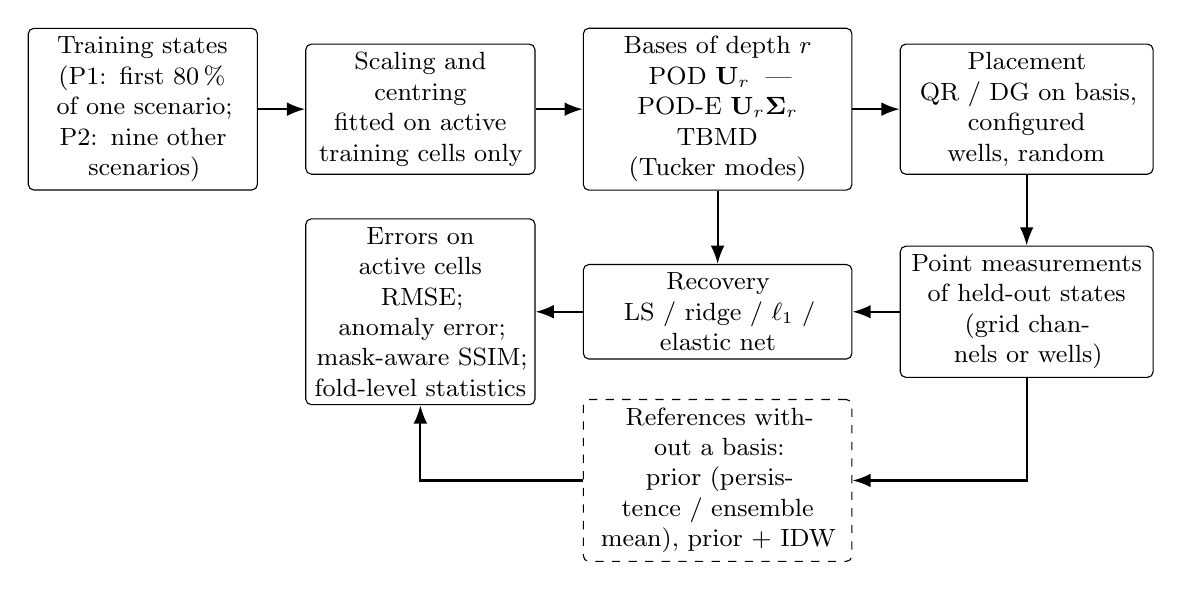
\begin{tikzpicture}[font=\small,>=Latex,node distance=4mm and 6mm,
  box/.style={draw,rounded corners=2pt,align=center,inner sep=3pt,minimum height=11mm,text width=27mm},
  ref/.style={box,dashed},
  arr/.style={->,thick}]
\node[box] (data) {Training states\\(P1: first 80\,\% of one scenario;\\P2: nine other scenarios)};
\node[box,right=of data] (norm) {Scaling and centring\\fitted on active\\training cells only};
\node[box,right=of norm,text width=32mm] (basis) {Bases of depth $r$\\POD $\mathbf{U}_r$ \;|\; POD-E $\mathbf{U}_r\boldsymbol{\Sigma}_r$\\TBMD (Tucker modes)};
\node[box,right=of basis,text width=30mm] (place) {Placement\\QR / DG on basis,\\configured wells, random};
\node[box,below=9mm of place,text width=30mm] (meas) {Point measurements\\of held-out states\\(grid channels or wells)};
\node[box,left=of meas,text width=32mm] (est) {Recovery\\LS / ridge / $\ell_1$ /\\elastic net};
\node[box,left=of est] (eval) {Errors on active cells\\RMSE; anomaly error;\\mask-aware SSIM;\\fold-level statistics};
\node[ref,below=5mm of est,text width=32mm] (refs) {References without a basis:\\prior (persistence / ensemble\\mean), prior + IDW};
\draw[arr] (data) -- (norm);
\draw[arr] (norm) -- (basis);
\draw[arr] (basis) -- (place);
\draw[arr] (place) -- (meas);
\draw[arr] (meas) -- (est);
\draw[arr] (basis.south) -- (basis.south |- est.north);
\draw[arr] (meas.south) |- (refs.east);
\draw[arr] (est) -- (eval);
\draw[arr] (refs.west) -| (eval.south);
\end{tikzpicture}}
\caption{Evaluation workflow. Nested runs select architecture, scaling, placement and recovery using scenario-grouped inner validation; E9 uses common measurements and a common paired solver. Everything above the measurement step is fitted on training states only; the held-out states enter only through the selected measurement rows and the final error computation. Dashed: references that use no reduced basis.}
\label{fig:workflow}
\end{figure}


The optimization study treats P2 as the outer protocol. For each held-out scenario, the other nine scenario identifiers are divided deterministically into three inner folds. Stage A selects representation, ranks, scaling and property architecture; Stage B selects recovery; Stage C selects placement; Stage D rechecks a bounded set of placement--solver combinations. The selected configuration is then refitted on all nine outer-training scenarios and evaluated once on the held-out scenario. The outer data never change a configuration within this run. Because earlier versions of the Brugge benchmark were inspected before this nested study, the design is post-development rather than a preregistered external validation.

\subsection{Experiment hierarchy}
\label{sec:exp_list}
The fixed-rank E1--E8 benchmark diagnoses representation, sensor budgets, noise, regularization, stability, cost and rigid property coupling. It includes POD, POD-E, TBMD, no-measurement priors and prior plus inverse-distance weighting; its full inventory and results are retained in Supplementary Sections~S4 and S9. V1/V3 verify the mathematical implementation. The nested optimization tests representation, recovery and placement using \OptValidationRecords{} sparse validation records and \OptOuterRecords{} outer records (Section~\ref{sec:optimization}). E9 then compares independent 3D with five 4D architectures at two coefficient capacities, with identical measurements and a common recovery solver (Section~\ref{sec:e9}). All comparisons retain ten P2 outer folds; random placements use 20 orders per fold.

\subsection{Metrics and statistics}
\label{sec:metrics}
All metrics use active cells after inverse transformation. Here $\mathbf X_k$ and $\widehat{\mathbf X}_k$ are the true and reconstructed active-cell-by-time matrices for property $k$. The broad E1--E8 benchmark retains export-unit $\mathrm{RMSE}_p$ (supplied export unit $u_p$) and $\mathrm{RMSE}_{S_o}$ ($-$). E9 adds two preregistered headline endpoints, separately for each property $k$. With outer-training ensemble mean $\boldsymbol\mu_{k,\mathrm{tr}}$ at the same cells and report steps,
\begin{equation}
E'_k=\frac{\lVert\widehat{\mathbf X}_k-\mathbf X_k\rVert_F}{\lVert\mathbf X_k-\boldsymbol\mu_{k,\mathrm{tr}}\rVert_F}.\label{eq:anomaly_error}
\end{equation}
Equation~\eqref{eq:anomaly_error}'s anomaly-relative denominator prevents the pressure datum from diluting error. Raw relative Frobenius error, train-range NRMSE and RMSE remain mandatory diagnostics.

E9 structural similarity is a mask-aware Gaussian SSIM of the same train-referenced anomalies. In every $7\times7$ window, Gaussian weights (standard deviation in grid-index units) are renormalised over active cells before the local mean, variance and covariance are computed. The centre must be active and active cells must contain at least half of the in-domain Gaussian weight. We use Gaussian standard deviation $1.5$, $K_1=0.01$, $K_2=0.03$ and a property-specific anomaly range fitted on outer training data. Inactive values therefore cannot increase the score. Local population moments use zero weight outside the array; scores are averaged over valid centres and report steps. Inner selection fits a separate reference and range on inner training only. Raw-field SSIM diagnoses ceiling effects; PSNR is omitted because it is a monotone transform of MSE under a fixed range.

Metrics are retained per outer fold and reported as mean, median, sample standard deviation and IQR. Paired comparisons use identical measurements and report steps, the number of favourable folds, and a two-sided Wilcoxon signed-rank diagnostic. E9 declares an empirical advantage only when the paired median is favourable and at least 7 of 10 folds improve. The related fixed-geology folds are not independent reservoir samples; unadjusted p-values are descriptive rather than population-level significance evidence.

\subsection{Implementation}
\label{sec:implementation}
All experiments use Python~3.12, NumPy, SciPy and TensorLy \cite{harris2020numpy,virtanen2020scipy,kossaifi2019}. On P2 fold 1, the first $r$ QR selections match the authors' public TBMD library as sets; ADMM differs by \VerStateDiff{} relatively on the first test snapshot (V1). This does not compare against Zhong et al.'s reference code. V3 checks explicit contractions, single-property reduction, active-cell ordering, measurement operators and rank-deficient least-squares invariance. Generated macros or tables supply every numerical claim.

AI-assisted tools supported the final audit of validation scripts, bibliography metadata and publication generators. Changes were checked by deterministic tests and regeneration from the retained outputs; final scientific interpretation and approval remain the authors' responsibility.

\section{Fixed-rank benchmark and representation limits}
\label{sec:results}
\label{sec:res_representation}
The original benchmark establishes the controls for the nested studies. Complete budget curves, fold comparisons, noise tests, temporal errors, sensor maps and timings are retained in Supplementary Section~S9. In the temporal hold-out protocol P1, persistence already achieves pressure RMSE \POnePriorGridTenP{} $u_p$, and no original TBMD configuration improves on it. We therefore emphasize P2, where the ensemble prior has pressure RMSE \PTwoPriorGridTenP{} $u_p$ and the held-out control scenario differs from the training ensemble.

With all active channels observed at the training-selected depth $r=\RankPTwoMin$, POD/POD-E reaches \EOnePTwoPodOracle{} $u_p$, whereas the original $(48,48,2)$ TBMD reaches \EOnePTwoTbmdOracle{} $u_p$. Increasing depth cannot remove this spatial-truncation floor. With full spatial ranks, the TBMD and POD-E subspaces agree to numerical precision, supporting Proposition~\ref{prop:tbmd_pod}.

Under sparse sensing, energy weighting and regularization matter independently of tensor order. At 30 grid channels, POD-E LS reaches \PTwoPodeLsGridThirtyP{} $u_p$. At all 30 existing joint wells, POD-E $\ell_1$ reaches \PTwoPodeLoneWellThirtyP{} $u_p$, versus \PTwoIdwWellThirtyP{} $u_p$ for prior plus interpolation and \PTwoTbmdLoneWellThirtyP{} $u_p$ for original TBMD. Least squares becomes unstable near the modal depth; regularization reduces this sensitivity. These stronger matrix and non-modal references are retained in the nested comparison below.

The matched E8 ablation also favours independent third-order property models over the original rigid joint model for both properties and both estimators at all wells (Supplementary Section~S4). E9 tests whether that negative result persists with partial sharing and structural metrics; it does not replace the E8 evidence.

\section{Nested TBMD optimization and Pareto regimes}
\label{sec:optimization}
Train-only rank selection reduces the original full-state pressure and saturation RMSE from \OptRepOriginalPressure/\allowbreak\OptRepOriginalSaturation{} to \OptRepJointPressure/\allowbreak\OptRepJointSaturation{} for joint ranks $(80,48,2,32)$. Independent property factors yield a lower equal-property normalized objective, but POD-E remains better for pressure alone. The accuracy and compression TBMD representations store \OptAccuracyCompression{} and \OptCompressionCompression{} times fewer values than rank-32 POD-E. Detailed rank, conditioning and ablation curves are in Supplementary Section~S7.

At all 30 existing joint wells, POD-E retains the lowest pressure and saturation errors (Table~\ref{tab:optimization_main}). Optimizing recovery on the original basis cannot remove its representation floor. Independent property models become poorly conditioned under sparse joint-well sensing, so their full-observation advantage does not imply a sparse advantage. Pressure-only measurements favour TBMD for pressure (\OptPressureWellThirtyCompressionPressure{} versus \OptPressureWellThirtyPodePressure{} $u_p$), while the independent saturation coefficients remain unobserved.

\begin{table}[htbp]\centering\small
\caption{Nested P2 reconstruction from all 30 existing joint-property wells (60 scalar channels); the prior uses no observations. Values are mean $\pm$ sample standard deviation over ten scenarios. Pressure uses export unit $u_p$ and saturation is dimensionless. Compression is the POD-E/TBMD factor-storage ratio. Bold marks the automatically determined smallest mean; method labels denote train-selected configurations.}
\label{tab:optimization_main}
\setlength{\tabcolsep}{3pt}
\begin{adjustbox}{max width=\textwidth}
\begin{tabular}{lrrr}\toprule
Method & Pressure RMSE & $S_o$ RMSE & Compression \\ \midrule
POD-E random & \textbf{0.084 $\pm$ 0.027} & \textbf{0.00057 $\pm$ 0.00013} & 1.00$\times$ \\
POD-E & \textbf{0.084 $\pm$ 0.027} & \textbf{0.00057 $\pm$ 0.00013} & 1.00$\times$ \\
Joint TBMD (tuned ranks) & 0.089 $\pm$ 0.023 & 0.00064 $\pm$ 0.00013 & 1.22$\times$ \\
TBMD compression & 0.175 $\pm$ 0.083 & 0.00065 $\pm$ 0.00012 & 2.62$\times$ \\
TBMD optimized & 0.179 $\pm$ 0.046 & 0.00064 $\pm$ 0.00013 & 2.12$\times$ \\
POD & 0.216 $\pm$ 0.123 & 0.00076 $\pm$ 0.00026 & 1.00$\times$ \\
Prior + IDW & 0.313 $\pm$ 0.165 & 0.00078 $\pm$ 0.00020 & -- \\
Original TBMD + tuning & 0.429 $\pm$ 0.051 & 0.00423 $\pm$ 0.00003 & 3.11$\times$ \\
Prior & 1.148 $\pm$ 0.558 & 0.00084 $\pm$ 0.00021 & -- \\
\bottomrule\end{tabular}\end{adjustbox}\end{table}


At 100 grid channels, optimized independent TBMD lowers the normalized joint error to \OptGridHundredAccuracyJoint{} from POD-E's \OptGridHundredPodeJoint. At 300 channels, the compressed model reaches \OptGridThreeHundredCompressionJoint{} versus \OptGridThreeHundredPodeJoint, with a lower joint objective in all ten folds. Pressure error remains higher; the gain is driven by saturation. Thus POD-E is preferred for existing joint wells and pressure accuracy, while TBMD offers a conditional accuracy--storage trade-off (Fig.~\ref{fig:opt_pareto}). Corrected cluster-constrained placement and all candidate baselines remain in the supplementary registry; clustering does not improve the 30-channel comparison.

\begin{figure}[tbp]
\centering
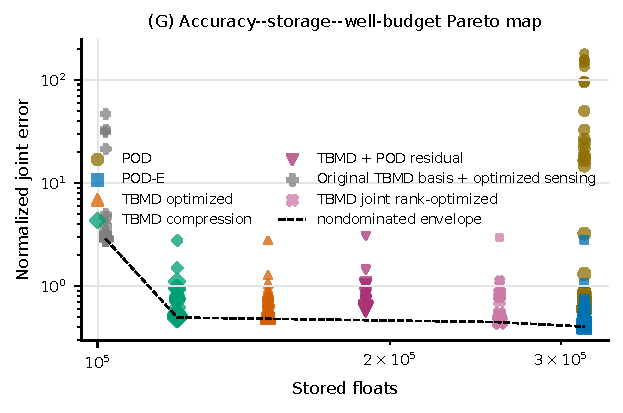
\includegraphics[width=\textwidth]{../../../studies/brugge_sparse_sensing/figures/fig14_pareto.pdf}
\caption{Accuracy--storage--well-budget map. Marker size increases with well budget; the dashed envelope contains nondominated mean points within the joint-well regime.}
\label{fig:opt_pareto}
\end{figure}

\section{What the explicit property mode contributes (E9)}
\label{sec:e9}

\subsection{Frozen dimensionality comparison}
E8 showed that the original rigid fourth-order model was worse than independent third-order property models in physical-unit RMSE. E9 retains that result and asks the narrower question for which TBMD was introduced: whether an explicit property axis improves relative field recovery or spatial structure when capacity, measurements and recovery are matched. Before computing any new E9 outer metric, we froze H1--H5, the anomaly-relative error and mask-aware anomaly SSIM in Section~\ref{sec:metrics}, two capacity controls, five fourth-order architectures, sensor budgets, a three-fold inner selection loss and the fold-consistency rule. The complete inner registry contains \ENineRepresentationRows{} representation and \ENineSparseRows{} sparse-recovery rows; all planned fits succeeded. Each of the \ENineOuterRows{} outer records was then generated in one pass over the frozen fold configurations.

Training-only dependence diagnostics support partial sharing: a common temporal direction coexists with weakly aligned property-specific spatial directions (Supplementary Section~S8). Full property rank adds no property compression.

\subsection{Current joint model versus optimized partial coupling}
The corrected metrics do not rescue the current rigid model: it meets the E9 advantage rule in only \ENineCurrentAdvantages{} of \ENineHeadlineComparisons{} headline comparisons. Its shared coefficients remain a severe restriction, especially for saturation. By contrast, train-only selection chooses 4D-B---shared spatial factors with separate property coefficients---in \ENineSharedHeadSelections{} of \ENineSparseSelections{} sparse fold/budget comparisons and in every full-observation comparison. Removing independent heads (4D-A/C) recreates the pressure--saturation compromise; property rank one is never selected for 4D-A.

With full observation and equal total capacity, optimized 4D lowers pressure anomaly error from \ENineFullThreeErrorP{} to \ENineFullFourErrorP{} and raises pressure anomaly SSIM from \ENineFullThreeSsimP{} to \ENineFullFourSsimP. Saturation error instead changes from \ENineFullThreeErrorSo{} to \ENineFullFourErrorSo, without a fold-consistent structural gain. The fourth-order representation therefore supplies a modest pressure and storage benefit (\ENineFullFourStorage{} versus \ENineFullThreeStorage{} stored floats), not universally better approximation.

Sparse observations produce the scientifically relevant gain. With 30 common grid channels, pressure/saturation anomaly error falls from \ENineGridThirtyThreeErrorP/\ENineGridThirtyThreeErrorSo{} to \ENineGridThirtyFourErrorP/\ENineGridThirtyFourErrorSo, while anomaly SSIM rises from \ENineGridThirtyThreeSsimP/\ENineGridThirtyThreeSsimSo{} to \ENineGridThirtyFourSsimP/\ENineGridThirtyFourSsimSo. Both properties and both endpoints meet the fold-consistency rule in both capacity controls. The same four-way advantage occurs at five existing wells. At 300 grid channels, the equal-total comparison remains favourable on all four endpoints (\ENineGridThreeHundredThreeErrorP/\ENineGridThreeHundredThreeErrorSo{} versus \ENineGridThreeHundredFourErrorP/\ENineGridThreeHundredFourErrorSo; SSIM \ENineGridThreeHundredThreeSsimP/\ENineGridThreeHundredThreeSsimSo{} versus \ENineGridThreeHundredFourSsimP/\ENineGridThreeHundredFourSsimSo). Intermediate well budgets and equal-per-property saturation error are more mixed; complete fold values and paired differences are retained in the canonical output.

% Generated by e9_analyze.py; do not edit.
\begin{table*}[htbp]\centering\small
\caption{E9 equal-total-capacity anomaly reconstruction: 32 coefficients per model, identical observations and common inner-selected solver. $E'$ is anomaly-relative error (lower is better); SSIM$'$ is mask-aware anomaly structural similarity (higher is better). Budget counts scalar channels for grid sensing and two-property wells for well sensing. Values are mean $\pm$ sample standard deviation over ten outer scenarios. 3D and 4D denote the independently train-selected models.}
\label{tab:e9_headline}
\setlength{\tabcolsep}{3pt}
\begin{adjustbox}{max width=\textwidth}
\begin{tabular}{lrlrrrr}\toprule
Geometry & Budget & Model & $E^\prime_p$ & $E^\prime_{S_o}$ & SSIM$^\prime_p$ & SSIM$^\prime_{S_o}$ \\ \midrule
grid & 30 & 3D & 1.167 $\pm$ 0.619 & 0.844 $\pm$ 0.287 & 0.406 $\pm$ 0.392 & 0.856 $\pm$ 0.034 \\
grid & 30 & 4D & 0.350 $\pm$ 0.162 & 0.465 $\pm$ 0.135 & 0.770 $\pm$ 0.254 & 0.932 $\pm$ 0.019 \\
grid & 300 & 3D & 0.148 $\pm$ 0.071 & 0.375 $\pm$ 0.114 & 0.941 $\pm$ 0.036 & 0.927 $\pm$ 0.026 \\
grid & 300 & 4D & 0.096 $\pm$ 0.039 & 0.348 $\pm$ 0.088 & 0.967 $\pm$ 0.021 & 0.948 $\pm$ 0.018 \\
wells & 5 & 3D & 0.498 $\pm$ 0.265 & 2.071 $\pm$ 0.378 & 0.818 $\pm$ 0.145 & 0.762 $\pm$ 0.011 \\
wells & 5 & 4D & 0.421 $\pm$ 0.287 & 0.950 $\pm$ 0.174 & 0.922 $\pm$ 0.039 & 0.866 $\pm$ 0.020 \\
wells & 15 & 3D & 0.212 $\pm$ 0.120 & 1.059 $\pm$ 0.242 & 0.939 $\pm$ 0.035 & 0.850 $\pm$ 0.029 \\
wells & 15 & 4D & 0.207 $\pm$ 0.092 & 0.890 $\pm$ 0.078 & 0.968 $\pm$ 0.016 & 0.868 $\pm$ 0.023 \\
wells & 30 & 3D & 0.191 $\pm$ 0.120 & 0.733 $\pm$ 0.154 & 0.920 $\pm$ 0.062 & 0.882 $\pm$ 0.032 \\
wells & 30 & 4D & 0.121 $\pm$ 0.092 & 0.722 $\pm$ 0.274 & 0.965 $\pm$ 0.035 & 0.894 $\pm$ 0.042 \\
\bottomrule\end{tabular}
\end{adjustbox}
\end{table*}


\begin{figure*}[htbp]
\centering
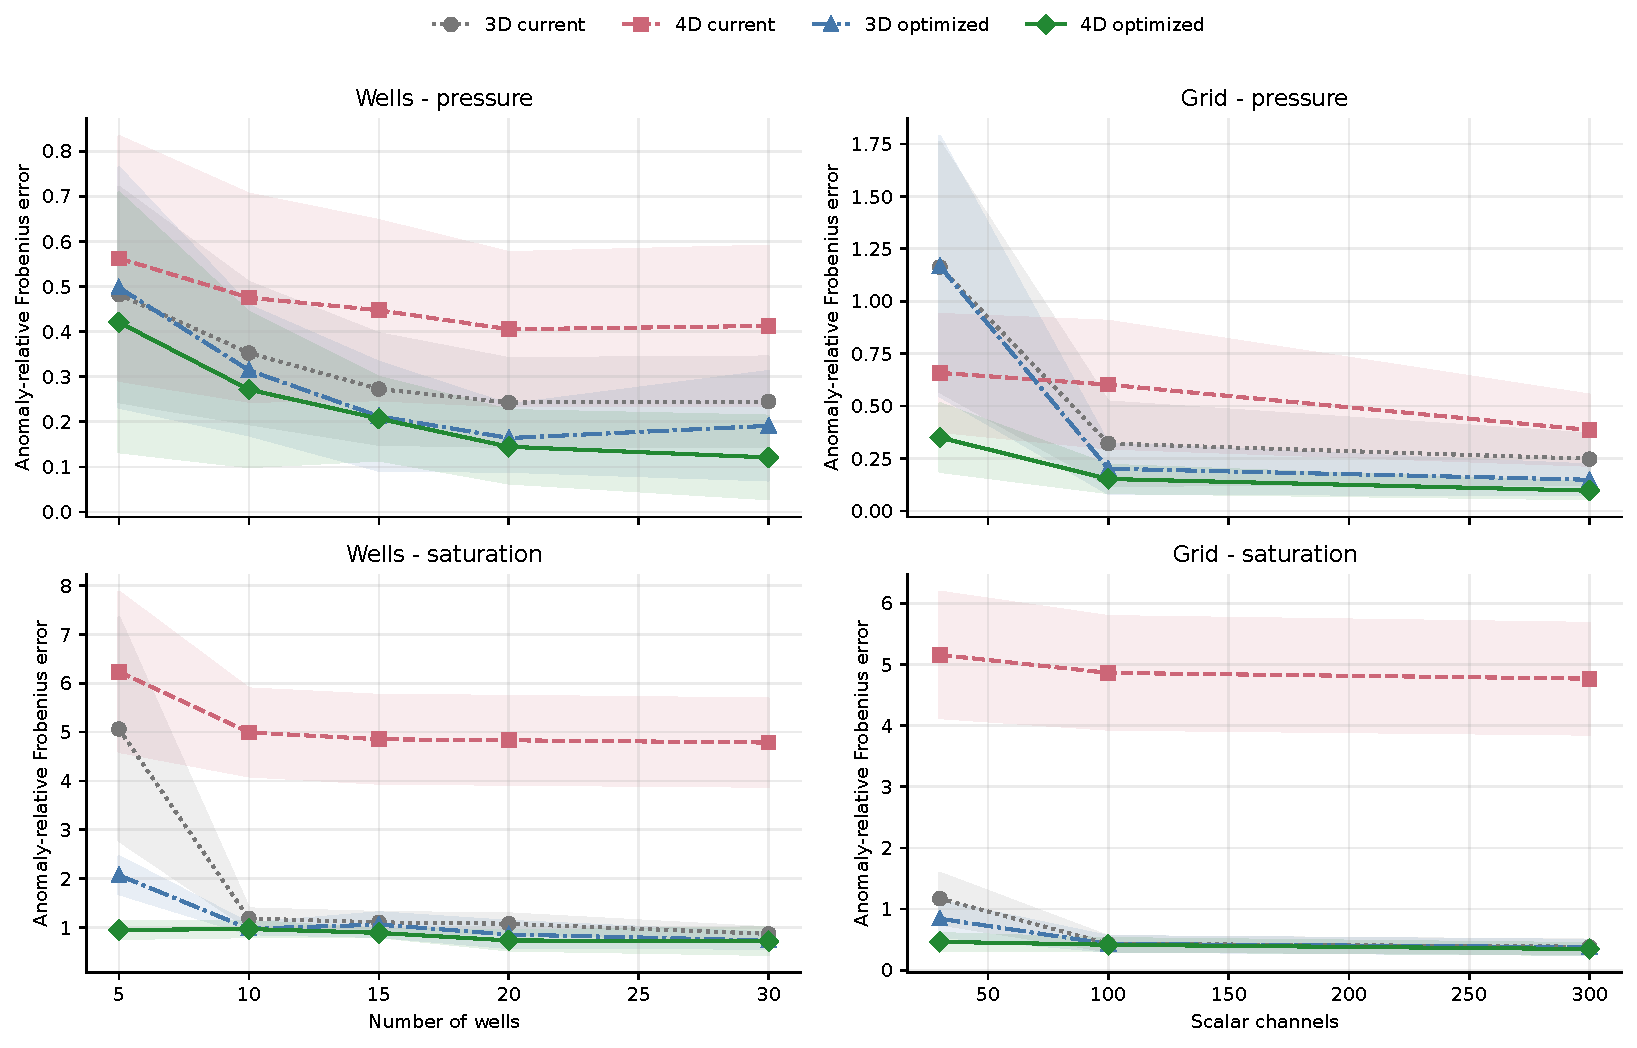
\includegraphics[width=\textwidth]{../../../studies/brugge_sparse_sensing/figures/fig15_e9_reconstruction_error.pdf}
\caption{E9 anomaly-relative reconstruction error against the common sensor budget under equal-total capacity. Curves show the current independent 3D/current rigid 4D pair and their train-selected counterparts. Every point is a mean over ten untouched outer folds; shaded bands show one sample standard deviation. Lower is better.}
\label{fig:e9_error}
\end{figure*}

\begin{figure*}[htbp]
\centering
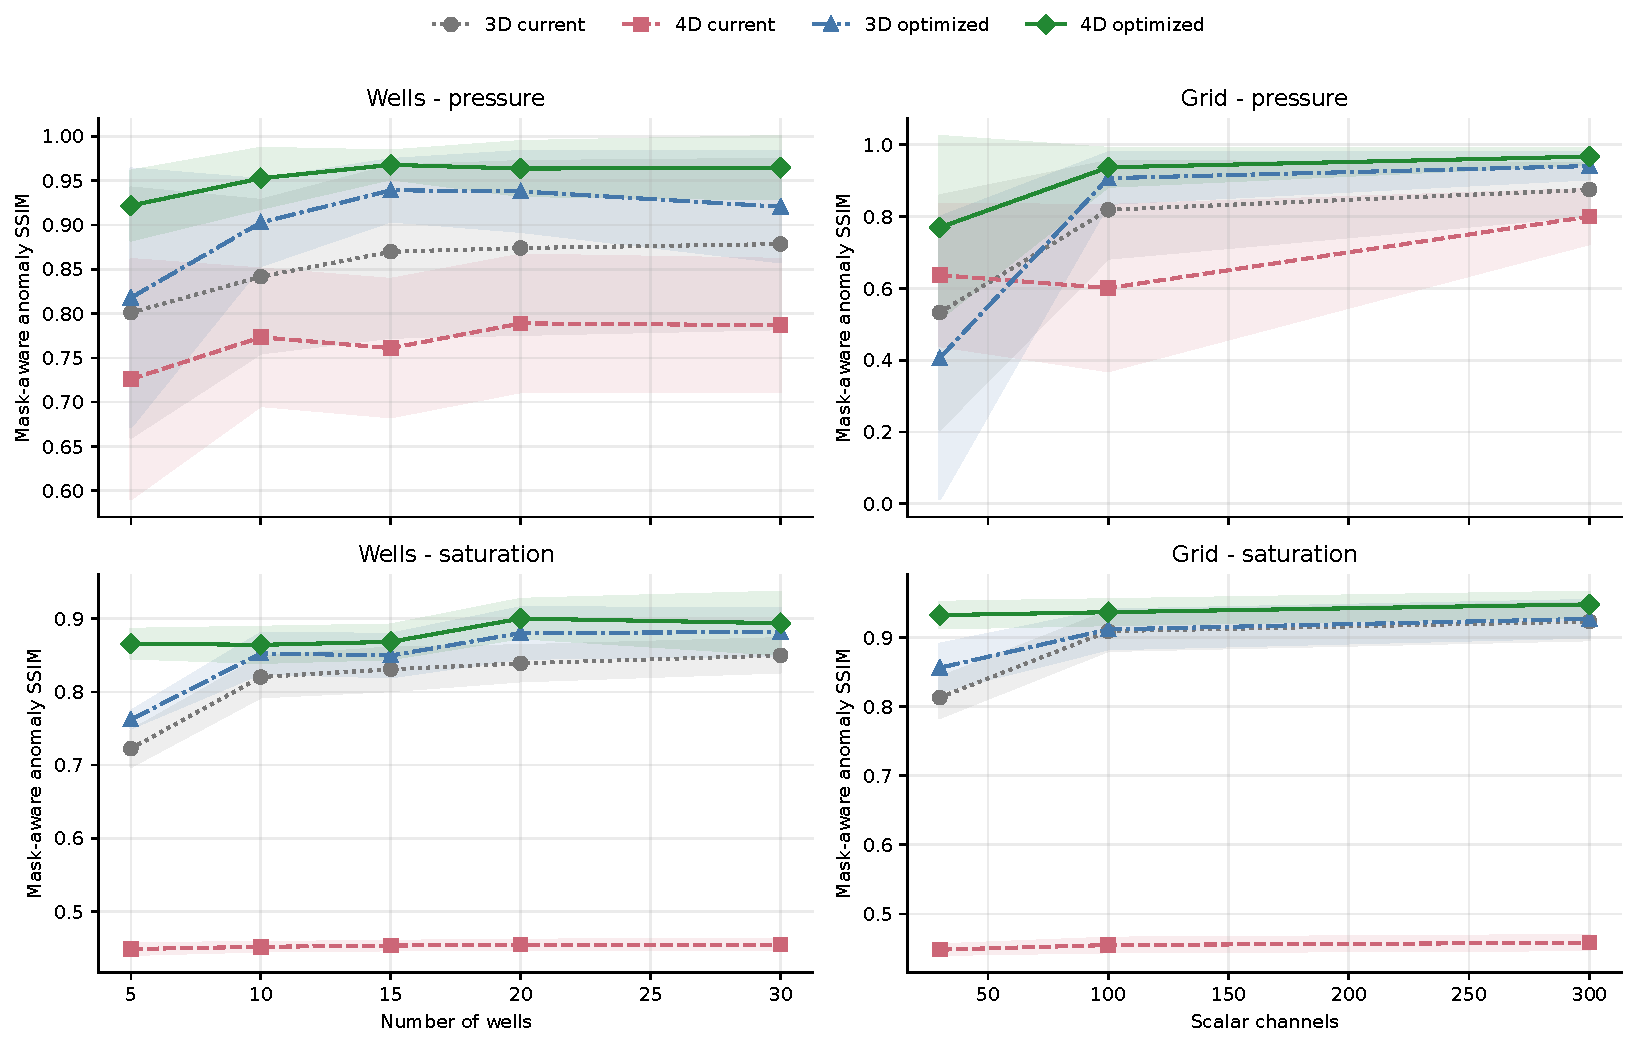
\includegraphics[width=\textwidth]{../../../studies/brugge_sparse_sensing/figures/fig16_e9_ssim.pdf}
\caption{Mask-aware anomaly SSIM for the same E9 comparisons. Panels show pressure (top) and oil saturation (bottom), versus well (left) or scalar grid-channel (right) budget; mean and one sample standard deviation across ten outer folds, equal-total capacity. Inactive background is excluded. Higher is better.}
\label{fig:e9_ssim}
\end{figure*}

\subsection{Metric concordance and structural fidelity}
RMSE, anomaly-relative error and anomaly SSIM rank the optimized pair identically in all but \ENineRankingDifferences{} of \ENineRankingRegimes{} property/regime comparisons. The exceptions bound the claim. At 15 wells under equal-total capacity, 3D has lower mean pressure RMSE (\ENineWellFifteenThreeRmseP{} versus \ENineWellFifteenFourRmseP), whereas 4D has lower anomaly error (\ENineWellFifteenThreeErrorP{} versus \ENineWellFifteenFourErrorP) and higher anomaly SSIM (\ENineWellFifteenThreeSsimP{} versus \ENineWellFifteenFourSsimP); only the SSIM gain satisfies the fold rule. At 300 grid channels under equal-per-property capacity, saturation pointwise metrics favour 3D but structural similarity favours 4D. These are structural-fidelity results, not restated accuracy wins.

Figure~\ref{fig:e9_maps} was fixed to scenario~1, report step 132 and 15 configured wells before outer evaluation. In that snapshot, 4D-B has higher pressure pointwise error but higher pressure anomaly SSIM, while it improves both saturation endpoints. The maps make the distinction between local structural preservation and absolute error visible.

\begin{figure*}[htbp]
\centering
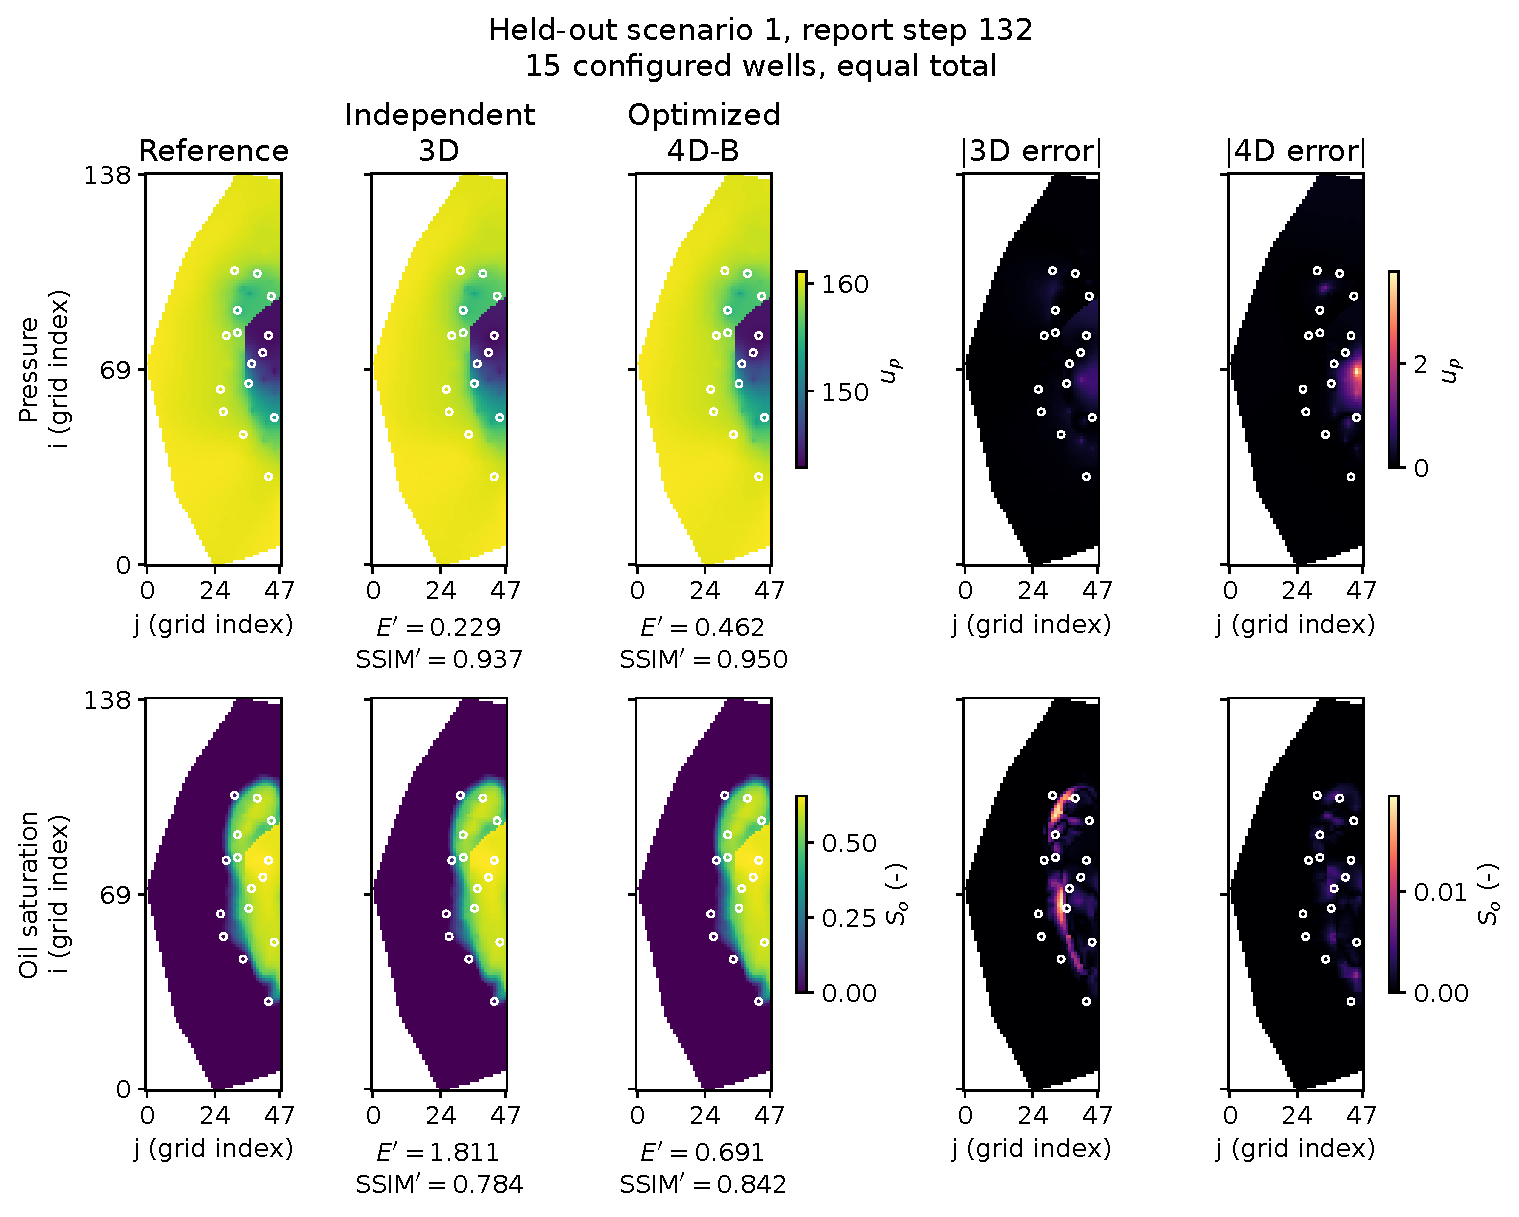
\includegraphics[width=\textwidth]{../../../studies/brugge_sparse_sensing/figures/fig19_e9_reconstruction_maps.pdf}
\caption{Fixed E9 reconstruction example. Columns show reference, independent 3D, train-selected shared-factor 4D-B, and matched absolute-error maps for pressure (top) and oil saturation (bottom). Axes are grid indices (no physical distances are available); white circles mark the 15 observed wells and inactive cells are blank. Pressure is in $u_p$ and saturation is dimensionless. All state panels share limits within each property, as do the paired absolute-error panels; panel annotations are snapshot-specific anomaly error and mask-aware anomaly SSIM.}
\label{fig:e9_maps}
\end{figure*}

The E9 advantage is conditional on coupling architecture, observation budget and metric. Shared-factor estimation can help sparse recovery; rigid coefficients, property rank one and full-state saturation approximation are not supported as general improvements.

\section{Discussion}
\label{sec:discussion}

\subsection{Why the methods behave as observed}
The fourth-order formulation creates an explicit property mode and spatial--property measurement operator. Matrix unfolding is lossless; the distinction from independent 3D is the imposed sharing, not avoidance of information loss during reshaping. E8 correctly found that rigid joint coefficients lose to independent property models. E9 shows why that result cannot be generalised to every fourth-order architecture: jointly estimated spatial factors with separate property coefficients improve many matched sparse comparisons, whereas the rigid model still fails. Property rank two adds no property compression; the gain comes from reusing spatial factors and regularising their estimation. Property rank one discards too much property-specific variation and is never selected for the rigid model.

The ensemble prior removes the common response, leaving a field-wide pressure shift and near-well deviations (Supplementary Section~S4). Energy weighting shrinks weak POD directions in underdetermined recovery; spatial truncation instead imposes an irreducible representation floor. Existing wells may leave the sampled basis nearly singular, so regularization trades variance for bias. Factor storage savings do not imply lower peak process memory because this implementation materialises the basis matrix.

\subsection{Implications for reservoir monitoring}
The benchmark gives four practical lessons. First, compare any sensing method with a no-measurement reference: persistence is strong in quasi-steady windows, and the P2 prior is exact initially. Second, a simulation-ensemble basis and existing-well measurements can recover the scenario-specific pressure deviation, but prior-plus-interpolation remains a necessary reference. Third, well ranking mainly protects unregularised least squares; it matters less with $\ell_1$ estimation. Fourth, saturation channels add little for this fixed-geology ensemble, and pressure-only fitting degrades saturation reconstruction. Cross-property inference therefore requires separate validation.

Grid-wide channels are idealised cell observations, not physical sensors or a performance bound for new wells. Their concentration near wells and high-variability regions (Supplementary Section~S9) only describes this ensemble.

\subsection{What optimization changes}
The nested study separates four conclusions that the fixed-rank benchmark could not. First, spatial rank is the dominant original TBMD limitation: solver and placement optimization on the old basis barely changes its all-well error, whereas rank expansion removes most of the representation floor. Second, completely independent property factors can give the best full-state equal-property objective, but create a poorly conditioned block basis under sparse sensing. Third, E9's shared-factor/independent-head model supplies a middle ground: it preserves property-specific coefficients while pooling spatial-factor estimation, with its clearest gain at five wells and 30 common grid channels. Fourth, tensor compression is real but not free. The compressed independent basis stores \OptCompressionCompression{} times fewer values than POD-E and has the better joint objective at 300 grid channels, while POD-E still has substantially lower pressure error and remains the preferred method for existing joint wells. These are architecture- and regime-specific statements, not overall leaderboard wins.

\subsection{Generality and relation to previous work}
The construction applies to co-registered variables: properties enlarge mode 3 without changing the derivation. Proposition~\ref{prop:tbmd_pod} shows why tensor order alone cannot guarantee an accuracy gain; ranks, sharing and atom scaling determine the representation. E9's pressure--saturation anomalies contain one strongly aligned global direction and many weakly aligned spatial directions, explaining why partial sharing succeeds where common coefficients do not. Gains reported elsewhere \cite{zhong2024tbmd,farazmand2023} may occur for different data structure or truncation. The Brugge conclusions require validation on other properties, grids and geological ensembles.

\section{Limitations}
\label{sec:limitations}
The study uses one reservoir model, an areal two-dimensional export, and ten control scenarios with fixed geology; it excludes geological uncertainty, three-dimensional layering and longer operating histories, and the leave-one-out folds are not independent reservoir samples. Time is available only as snapshot indices, and the P2 prior assumes time-aligned training-ensemble trajectories. Measurements are idealised cell values: well-bore effects, gauge drift, correlated errors and saturation-measurement difficulty are not modelled beyond additive Gaussian noise; E9's headline comparison is noise free. The optimization is nested within P2, but the Brugge benchmark and prior outer results had already informed the diagnosis and bounded search; the outer folds are untouched within this run, not an externally preregistered data set. Anomaly-relative error and mask-aware SSIM are declared scientific choices; another application may prefer a different reference state, window or property weighting. The exploratory coupling--gain associations have only ten paired folds and do not identify a causal threshold. Model storage is measured exactly, whereas method-specific peak process memory is not. Kriging, neural decoders \cite{fukami2021,zou2025prosnet} and ensemble data assimilation \cite{evensen2009} were not included as baselines. Unrestricted public redistribution of the transformed TNO-based state exports has not been established; the corresponding author can instead provide them upon reasonable request, subject to applicable data-use and access conditions. Released result files support checking every table, statistic and quoted number (data availability statement).

\section{Conclusions}
\label{sec:conclusions}
Sparse reconstruction on the Brugge control ensemble depends on tensor truncation, property sharing and observability rather than tensor order alone. Rank expansion removes much of the original TBMD representation floor. Shared spatial factors with separate property coefficients improve matched anomaly-error and structural-similarity comparisons most clearly at five wells and 30 common grid channels; rigid joint coefficients and property rank one do not provide a general advantage. Full-observation gains are limited to pressure, and metric-dependent cases must remain qualified.

POD-E retains the lowest errors at all existing joint-property wells and stronger grid-sensing pressure accuracy. Compressed independent TBMD instead offers a lower joint objective at high grid budgets, driven by saturation, with lower stored-factor size. These conditional trade-offs support choosing representations against the target property and measurement regime, not a universal method ranking. Frozen outer refits support numerical repeatability, while geological ensembles, three-dimensional states, realistic well responses and external observations remain necessary to establish transferability.

\section*{Computer code availability}
\label{sec:availability}
\noindent\emph{Name:} TBMD library with the Brugge sparse-sensing study package (\texttt{studies/brugge\_sparse\_sensing}). \emph{Developer and contact:} Denis Samatov, National Research Tomsk Polytechnic University, dss53@tpu.ru. \emph{Year first available:} 2026. \emph{Hardware:} CPU, about 2\,GB per parallel job; no GPU. \emph{Software:} Python~3.12, exact packages in \texttt{requirements-lock.txt}. \emph{Language:} Python. \emph{Code licence:} MIT, excluding third-party data. \emph{Access:} \url{https://github.com/denis-samatov/tensor-based-modal-decomposition-method}. The previous release v2.1.0 (\CodeArchiveDOI{}) predates the final E8/V3, nested-optimization and E9 additions. The present revision is prepared for release as v2.2.0; public tag creation and archival DOI assignment remain pending. \emph{Reproduction:} \texttt{run\_tbmd\_optimization.sh} validates the checksummed HDF5/JSON inputs, runs the broad nested optimization and independently refits frozen configurations; \texttt{run\_e9\_property\_mode.sh} performs or independently reproduces the frozen third- versus fourth-order study and regenerates its metrics, tables and figures; \texttt{run\_all.sh} retains the earlier benchmark chain and \texttt{verify\_outputs.sh} checks stored legacy, nested-optimization and E9 outputs. None reconstructs the input exports from the original t-Navigator deck.

\section*{Data availability}
The t-Navigator simulations analysed in this study are represented by two supplied, transformed inputs for ten Brugge well-control scenarios: \path{data_exp_4_.h5} (pressure and oil-saturation arrays) and \path{all_wells_exp_4.json} (well coordinates). The archive contains neither the original deck nor the exporter and vertical-reduction configuration, so original model-to-HDF5 reproduction is unavailable. The transformed data supporting the findings of this study are available from the corresponding author upon reasonable request, subject to the applicable data-use and access conditions. The transformed input files cannot be deposited publicly because of institutional access conditions. Requests should be directed to the corresponding author and will be considered under those conditions. They are not distributed under the code repository's MIT licence. Their SHA-256 checksums are given in Supplementary Table~S1 and verified before computation. The release candidate contains the derived performance metrics, statistics, tables, number macros and figures required to check the article.

\section*{CRediT authorship contribution statement}
\textbf{Denis Samatov:} Conceptualization, Methodology, Software, Validation, Formal analysis, Investigation, Visualization, Writing -- original draft. \textbf{Boris Merzlikin:} Supervision, Methodology, Writing -- review \& editing. \textbf{Gleb Shishaev:} Data curation, Validation, Writing -- review \& editing.

\section*{Declaration of competing interest}
The authors declare that they have no known competing financial interests or personal relationships that could have appeared to influence the work reported in this paper.

\section*{Funding}
The research was supported by the program of the National Research Tomsk Polytechnic University (Prioritet-2030-ISP-032-090-2026). The funder participated in data collection, interpretation of the results, and the decision to submit the manuscript for publication.

\section*{Acknowledgements}
The authors acknowledge TNO for making the Brugge benchmark data set available.

\section*{Declaration of generative AI and AI-assisted technologies in the manuscript preparation process}
During the preparation of this work, the authors used OpenAI GPT-4o and OpenAI GPT-5-Codex to assist with manuscript drafting, language and text editing, and submission-package consistency checks. After using these tools, the authors reviewed and edited the content as needed and take full responsibility for the content of the publication. AI assistance also supported source-code review and corrections to publication generators and validation scripts; it is not an independent scientific validation. Reported numerical results were produced by the documented Python workflow on the checksummed inputs, and the figures were rendered by repository scripts rather than a generative image model.


\bibliographystyle{elsarticle-num}
\bibliography{references}

\end{document}
